% Ergebnisse - Endergebnisse der Arbeit, Performance, Bilder (auf dpi achten, mind. 300), Kennkurven, Warps, weitere Leistungsmessungen bez. auf meine Arbeit
% -> ggf. Results and Discussion seperat halten
% Bedeutung der Ergebnisse (im Rahmen dessen was wissenschaftlich haltbar ist)
\chapter{Ergebnisse und Diskussion}\label{chap::resdisc}
In den Ergebnissen werden die verschiedenen Raycast Methoden auf Bildqualität und Performanz untersucht.
Anschließend folgt eine Diskussion bezüglich der verschiedenen Ergebnissen.

\section{Ergebnisse}\label{sec::results}
Der erste Abschnitt beinhaltet Ergebnisse der Implementierungen des Standard Raycasts, \emph{MDC} \ref{ss::MDC} und \emph{DDC} \ref{ss::DDC} sowie der Implementierung der Variierung der Strahlabtastrate \ref{sec::workpacks::ors}.
Dabei liegt der Fokus auf die Beschreibung der wahrgenommenen Bildqualität der verschiedenen Methoden.
Der zweite Abschnitt beinhaltet gemessene Performanzleistungen der jeweiligen Implementierungen bei der Verwendung unterschiedlicher Transferfunktionen und Volumendaten.
Die verschiedenen Methoden werden hier im Hinblick auf die benötigten Ausführungszeiten bei Berechnungen mit verschiedenen Volumen verglichen.

\subsection{Bildqualität}
Für die Bildqualität werden Screenshots von Berechnungen mit unterschiedlichen Raycast Methoden vorgestellt, bewertet und verglichen.
Die Bewertung erfolgt anhand der wahrgenommenen Bildqualität und wie diese sich verändert, wenn die Bildabtastrate und die Strahlabtastrate variiert werden.
Es wird von drei Methoden die Bildqualität untersucht, wobei diese jeweils Ergebnisse mit unterschiedlichen Bildabtastraten produzieren.
Diese sind: Standard-, \emph{MDC}- und \emph{DDC}-Methode.
Die Bildqualität dieser Methoden wird einmal mit konstanter Strahlabtastrate und einmal mit variierte Strahlabtastrate vorgestellt.
Dafür werden zwei Volumen verwendet, wobei die Ergebnisse des ersten Volumens für die unterschiedlichen Methoden getrennt-, und die Ergebnisse mit dem zweiten Volumen im Anschluss für einen besseren Vergleich zusammen vorgestellt werden.
% Für jedes der Volumen wird jeweils das Bild in normaler Auflösung, welche mit der ursprünglichen Implementierung berechnet wurde sowie das Ergebnis der Berechnung des Bildes durch \emph{MDC} und \emph{DDC} gezeigt.
% Bei den Berechnungen durch \emph{MDC} und \emph{DDC} werden die jeweils verwendeten Parameter der Berechnung angegeben.

Die Ergebnisse in diesem Abschnitt wurden alle mit einer Auflösung von $2263\times1306$\,Pixel berechnet.
Alle Abbildungen, die das selbe Volumen zeigen, wurden mit der gleichen Transferfunktion und aus der gleichen Perspektive berechnet.
Die Unterschiede bei der Berechnung ergeben sich ausschließlich aus einer veränderten Bild- oder Strahlabtastrate.

Der Begriff \emph{maximale Bildabtastrate} bezieht sich auf die Bildabtastrate mit einem Wert von circa $1$ und bedeutet, dass für jeden Pixel des Bildes ein Strahl berechnet wurde, der den Farbwert des Pixels angibt.
Eine Bildabtastrate von $\frac{1}{2}$ bedeutet, dass in x- und y-Richtung nur für jeden zweiten Pixel ein Strahl berechnet wurde.
Eine Bildabtastrate von $\frac{1}{7}$ bedeutet, dass in x- und y-Richtung nur für jeden siebten Pixel ein Strahl berechnet wurde.
Die Bildabtastrate kann theoretisch aber auch auf einen Wert größer als $1,0$ gesetzt werden.
In allen Berechnungen, außer bei der Methode \emph{MDC}, wurde die maximale Bildabtastrate $1,0$ gewählt.
Aufgrund der Implementierung und der verwendeten Auflösung für die Berechnungen ist die Bildabtastrate für die Methode \emph{MDC} nur $0,96$.
Dies wird bei der Bewertung aber wie eine Bildabtastrate von $1,0$ behandelt. 

Die Strahlabtastrate gibt an, in welchem Abstand ein Strahl abgetastet wird.
Die Abtastdistanz wird mit $\frac{1\times Voxellaenge}{maximale Strahlabtastrate}$ berechnet.
Die Voxellänge ergibt sich aus der Skalierung der Voxel, welche abhängig von den verwendeten Volumen ist.
In allen Berechnungen ist die maximale Strahlabtastrate $1,5$ gewählt worden.

Wurde eine Abbildung mit variierter Strahlabtastrate berechnet, so bedeutet dies, dass die Strahlabtastrate an der Mausposition den maximalen Wert der Strahlabtastrate hat.
Mit zunehmender Distanz zur Mausposition nimmt die Strahlabtastrate dann bis auf einen Wert von $\frac{maximale Strahlabtastrate}{4}$ ab.

Das erste Volumen ist ein ct-scan eines Bonsai.
Das Volumen hat eine Auflösung von $256\times256\times256$\,Voxel.
Die Slice-Dicke der einzelnen Voxel ist $1,0\times1,0\times1,0$ und gibt die Skalierung der einzelnen Voxel an.
Das heißt, dass die Voxel in x-, y- und z-Richtung hier eine einheitliche Skalierung haben.
% Anders als das erste Volumen, welches ein ct-scan ist, ist das zweite Volumen ein Zeitschritt aus der Simulation einer \emph{shock wave formation in core-collapse supernova} von John Blondin, NCSU.
% Es hat eine Auflösung von $432\times432\times432$\,Voxel, welche ebenfalls in x-, y- und z-Richtung eine Skalierung von $1,0$ haben.
% Die Dichte der Voxel gibt die physikalische Entropie an der Position in der Simulation an.

\subsubsection{Standard Raycast}\label{ss::res::sr}
% \todo{Die gleiche Transferfunktion verwenden, wie die, womit die Daten gemessen wurden.}; ggf. auch dazu Daten messen.
Abbildung \ref{fig::res::bon_st} zeigt eine Berechnung des Volumens \emph{Bonsai} mit dem Standard Raycast.
Die Bildabtastrate ist bei der Berechnung des Standard Raycasts im ganzen Bild homogen und hat den Wert $1$.
Das heißt, dass für jeden Pixel des Bildes ein Work-Item gestartet wurde, um den Raycast eines Strahls zu berechnen.
Der jeweilige Pixel erhält die berechnete Farbe des Work-Items.

Durch die Interpolation der Voxel wird das Volumen mit weichen Konturen und Flächen gezeichnet.
Die Transferfunktion hebt die Voxel mit etwas höherer Dichte farblich hervor.
Dies entspricht hier dem Stamm und den Ästen sowie der Erde und der Schale, in welcher sich der Bonsai befindet.
Die Blätter werden teilweise ausgeblendet.
Die Voxel, die nicht zu dem Bonsai Objekt gehören, zum Beispiel Leerräume, haben teilweise auch Dichtewerte größer null.
Daher wurde die Transferfunktion so gewählt, dass diese ausgeblendet sind.
Insgesamt werden die Flächen aber transparent gezeichnet, so dass auch eigentlich verdeckte Strukturen zu sehen sind.

Wie in den Grundlagen im Abschnitt \ref{sec::eye} zum visuellen Wahrnehmungssystem beschrieben wurde, kann man feststellen, dass wenn ein bestimmter Punkt in der Abbildung \ref{fig::res::bon_st} fokussiert wird, die vom Blickpunkt entfernten Bereiche unscharf erscheinen.
Im Standard Raycast werden auch diese mit normaler Bildabtastrate gezeichnet, obwohl dies aufgrund der Limitierungen des visuellen Wahrnehmungssystems, eigentlich nicht notwendig ist.

% Abbildung \ref{fig::res::sup_st} zeigt eine Berechnung des Volumens der Supernova im Zeitschritt $1353$. ; Supernova wird am Ende der Bildqualität zusammengefasst
% Das Bild wurde mit dem Standard Raycast berechnet, so dass die Bildabtastrate in dem gesamten Bild gleich ist.
% Dies wird auch durch die Vergrößerung von Bereichen an unterschiedlichen Positionen innerhalb der Abbildung verdeutlicht.
% Die Strahlabtastrate hat einen Wert von $1,5$ und die Interpolation der Voxel ist aktiviert.
% Die Transferfunktion wurde so gewählt, dass das Volumen als ganzes transparent erscheint aber Bereiche mit den selben Dichtewerten farblich gruppiert und hervorgehoben wurden.

\begin{landscape}
	\begin{figure}
		\centering
		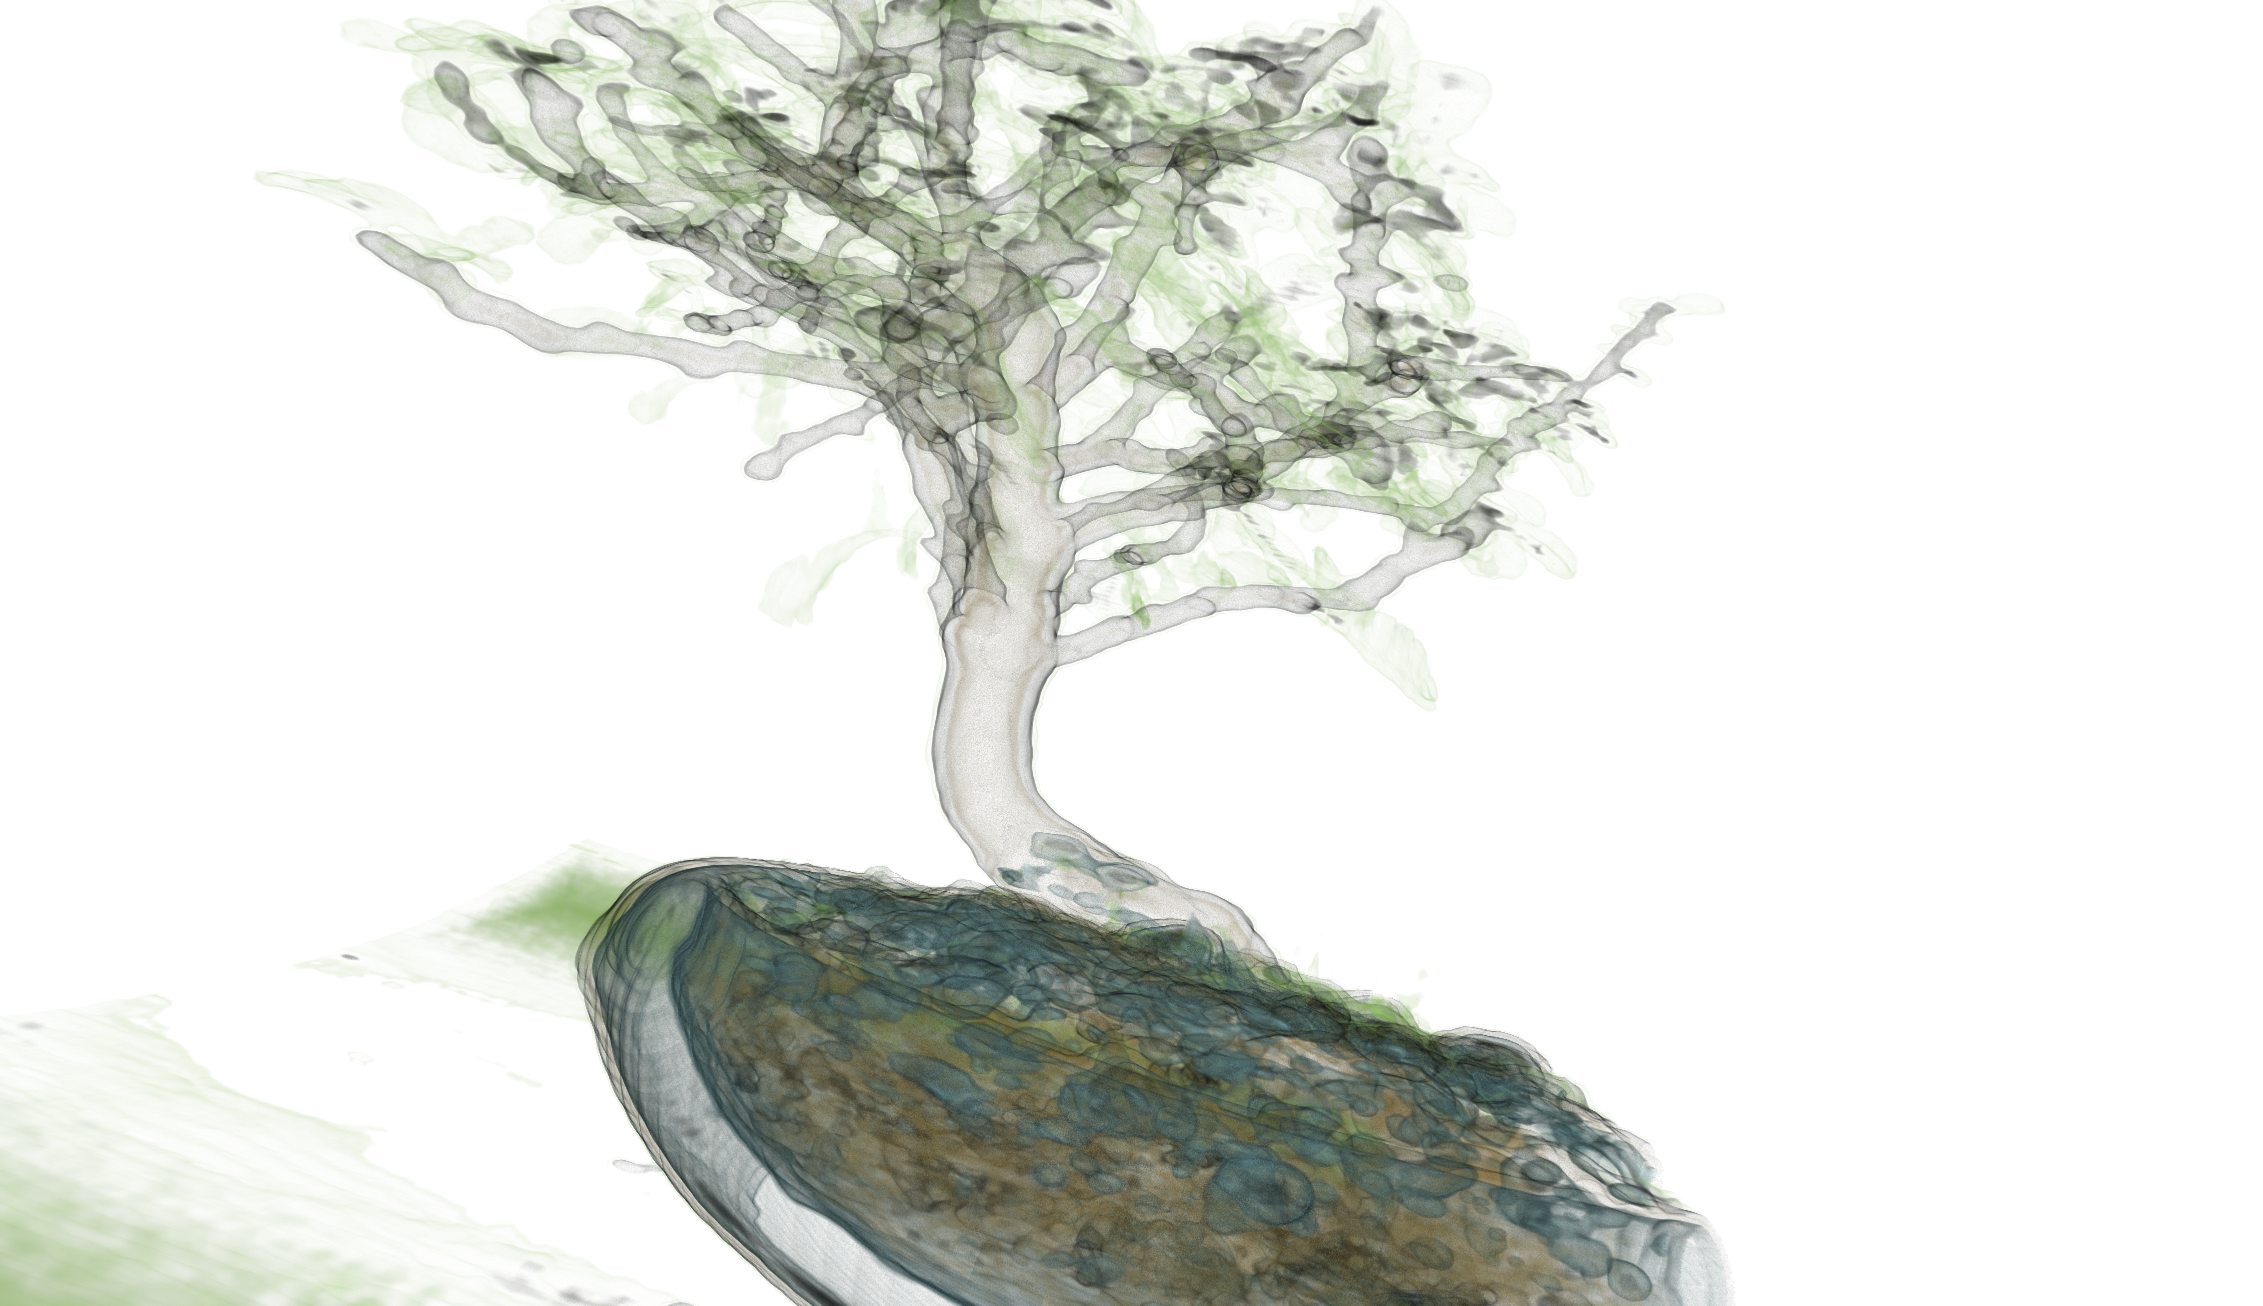
\includegraphics[width=\textheight]{../../Neue_Messungen/Bonsai/st.png}
		\caption{Volumen Bonsai mit ursprünglichem Raycast berechnet. Das Bild hat eine Bildabtastrate von $1$ und eine Strahlabtastrate von $1,5$.}
		\label{fig::res::bon_st}
	\end{figure}
\end{landscape}

\begin{landscape}
	\begin{figure}
		\centering
		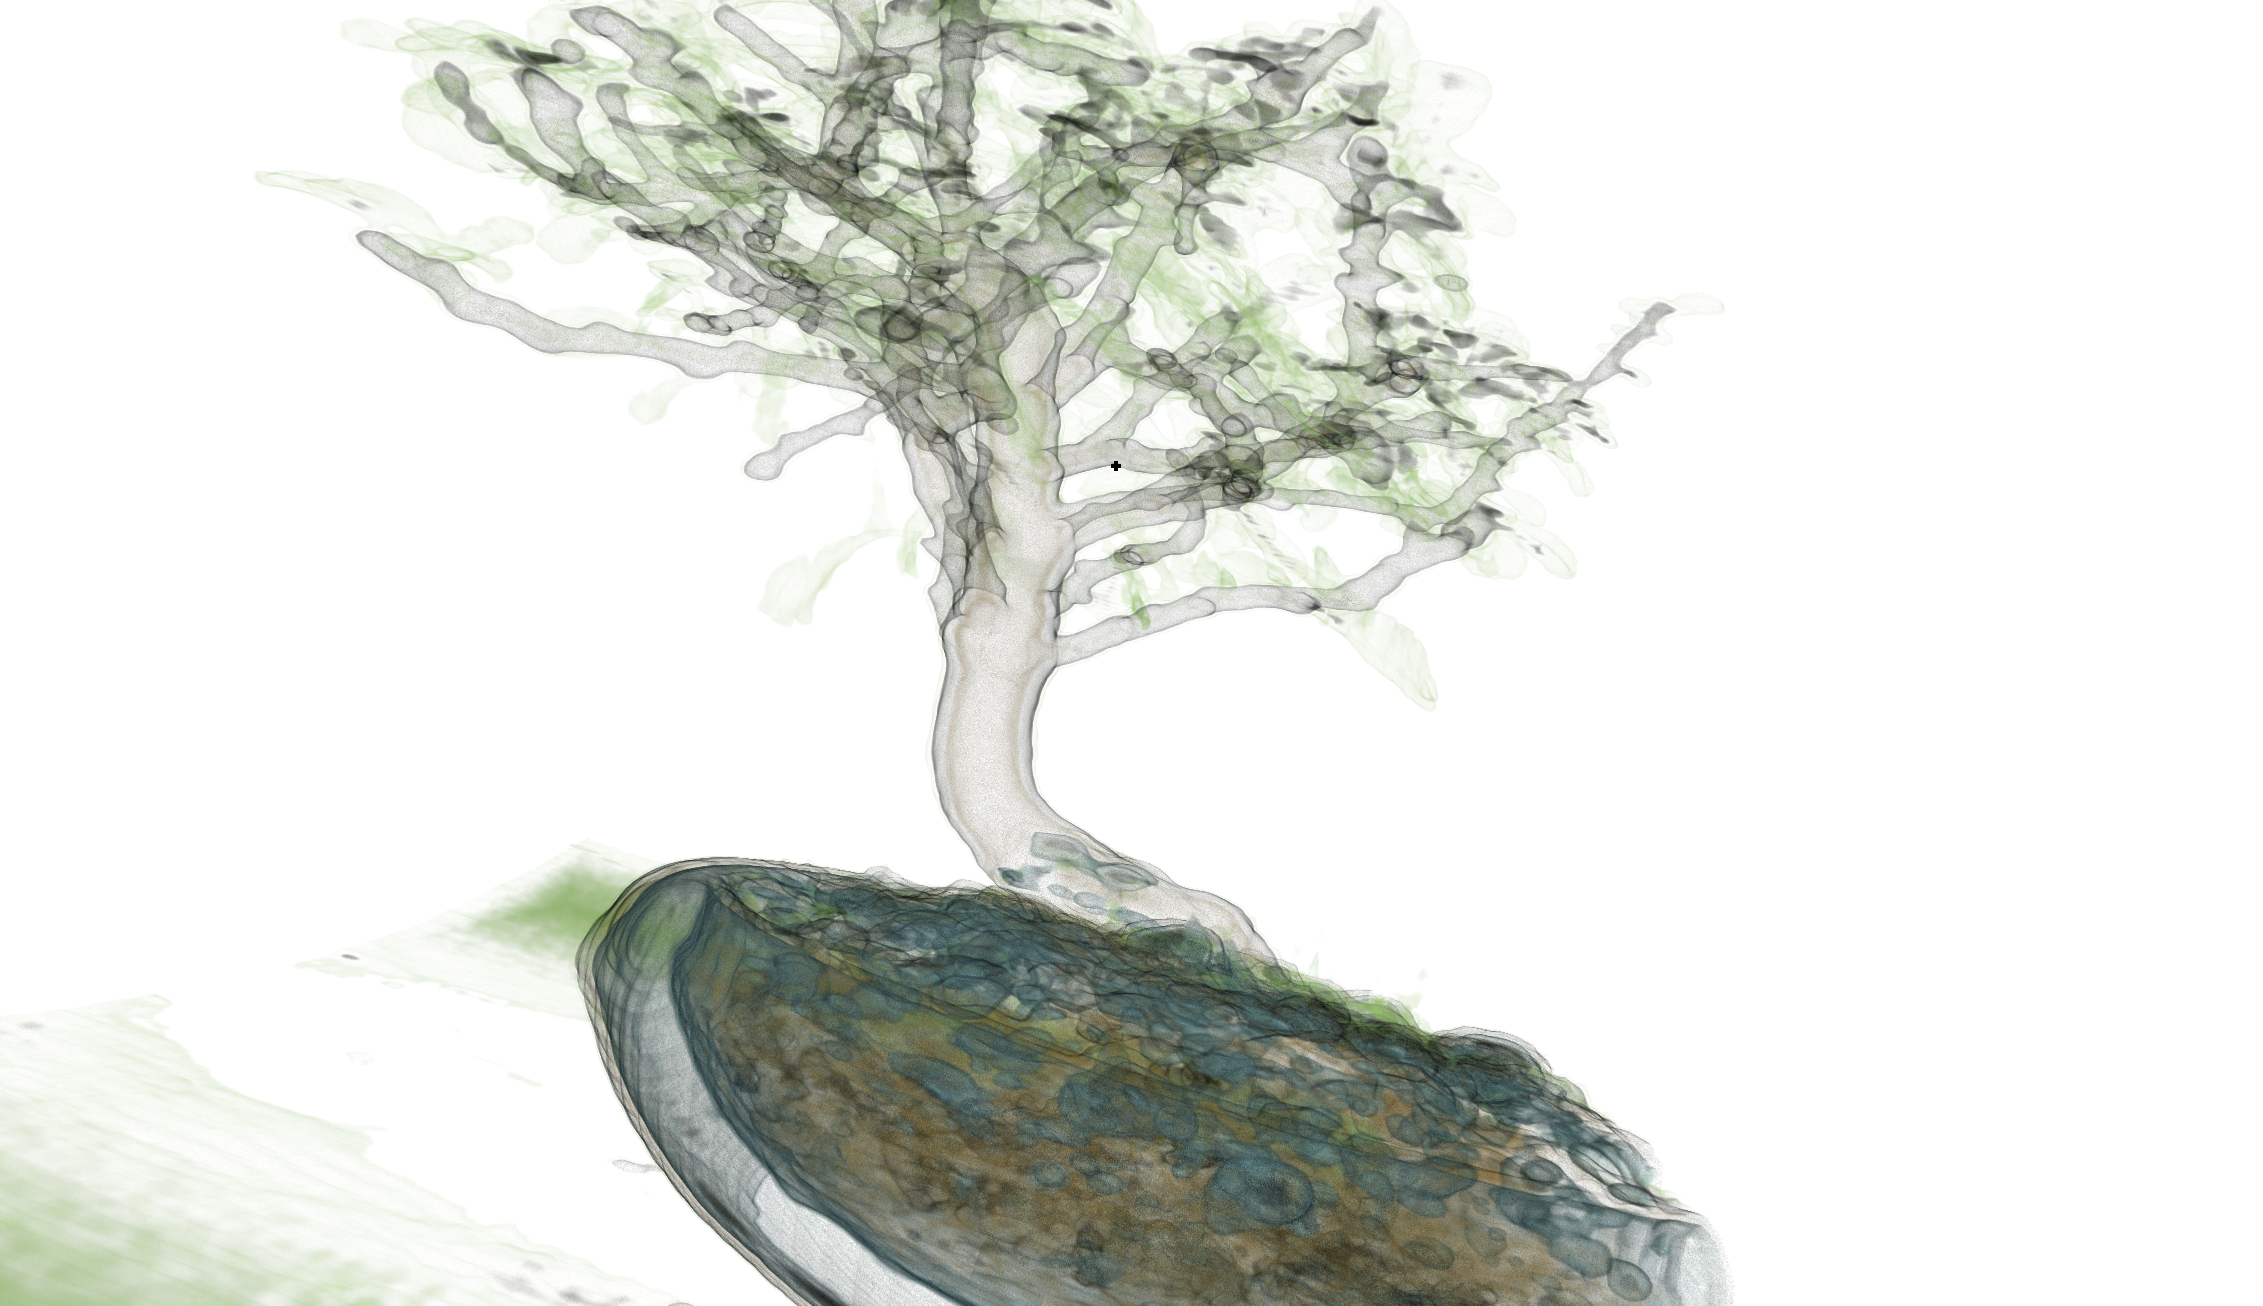
\includegraphics[width=\textheight]{../../Neue_Messungen/Bonsai/st_ors.png}
		\caption{Volumen Bonsai mit modifizierten Standard Raycast berechnet. Die Bildabtastrate beträgt $1$. Die Strahlabtastrate hat an der Mausposition einen Wert von $1,5$ und nimmt, abhängig von der Distanz zur Mausposition, bis zu einem Wert von $\frac{1,5}{4}$ ab.}
		\label{fig::res::bon_st_ors}
	\end{figure}
\end{landscape}

\subsubsection{MDC Raycast}\label{ss::res::mdc}
Der \emph{MDC} Raycast ist das Ergebnis des Arbeitspakets, aus dem Abschnitt \ref{ss::MDC}.
Die Abbildung \ref{fig::res::bon_mdc} zeigt das Volumen \emph{Bonsai}, welches mit dem \emph{MDC} Raycast erstellt wurde.
Das Bild wurde dabei aus der selben Perspektive und mit der gleichen Transferfunktion berechnet, wie dies auch in Abbildung \ref{fig::res::bon_st} der Fall war.
Die Strahlabtastrate ist ebenfalls gleich wie bei der Berechnung des Bildes in Abbildung \ref{fig::res::bon_st}, welches mit dem Standard Raycast berechnet wurde.
Die maximale Bildabtastrate in Abbildung \ref{fig::res::bon_mdc} hat einen Wert von $0,96$ statt einem Wert von $1,0$.
Damit wird einer leichten Verschiebung des Bildes, aufgrund der zwei unterschiedlichen Bildabtastraten, entgegengewirkt.
Die Anpassung der Bildabtastrate muss aber je nach Auflösung des Bildes leicht variiert werden.

In diesem Fall, beim \emph{MDC} Raycast, wurden zwei Bilder berechnet, welche anschließend passend zusammengefügt wurden.
Das erste Bild wurde mit nur einem viertel der Auflösung berechnet und anschließend auf die ursprüngliche Auflösung interpoliert.
Das zweite Bild wurde mit der ursprünglichen Auflösung berechnet, dafür aber nur ein rechteckiger Ausschnitt an der Mausposition.
Anschließend wurde das zweite Bild an der Mausposition in das auf die normale Auflösung interpolierte erste Bild eingefügt.

\todo{Mausposition in das Bild einzeichnen.}
An den Konturen der Abbildung \ref{fig::res::bon_mdc} ist ein leichter Abfall der Auflösung des Bildes zu erkennen.
Die Konturen, welche in Abbildung \ref{fig::res::bon_st} noch weich gezeichnet wurden, haben außerhalb des Rechtecks um die Mausposition nun Artefakte der Unterabtastung, wie zum Beispiel leichte Treppenstufen.
Innerhalb des Rechtecks sind die Konturen immer noch weich gezeichnet und es ist dort kein Unterschied zu Abbildung \ref{fig::res::bon_st} zu sehen.

Die Größe des Rechtecks beträgt $?$\,Pixel in x- und y-Richtung und ist groß genug, dass die Abnahme der Auflösung im äußeren Bereich kaum auffällt.
Wird bei aktivem Eyetracking anstelle der Mausposition die Blickposition verwendet, so ist der aktuell betrachtete Bereich immer hoch aufgelöst.
Ein Unterschied zwischen den beiden Bereichen fällt während einer Fokussierung kaum auf.
Wenn der Fokus langsam über das Bild wandert, kann man einen Unterschied zwischen den Auflösungen erkennen.
An dem Übergang des normal aufgelösten Bereichs zu dem Bereich mit der halben Auflösung kommt es während einer Bewegung an den Konturen des Volumen zu leichten Veränderungen.
Diese können die Aufmerksamkeit auf sich ziehen und daher leicht störend wirken.

Obwohl der Bereich außerhalb des Rechtecks mit nur einem Viertel der Bildabtastrate innerhalb des Rechtecks berechnet wurde, ist die Bildqualität in diesem Bereich noch recht gut.
Da die Sehschärfe mit zunehmenden Winkel von der Fovea weg immer weiter abnimmt, könnte die Bildabtastrate außerhalb des Rechtecks vermutlich weiter gesenkt werden, ohne dass dies die Bildqualität bei der Verwendung eines Eye-Trackers beeinträchtigt.

% Das Bild in Abbildung \ref{fig::res::sup_mdc} wurde ebenfalls mit dem \emph{MDC} Raycast berechnet und anschließend bearbeitet. ; Direkter Vergleich
% Es zeigt einen Zeitschritt in einer Simulation von einer Supernova.
% Die Bild- und Strahlabtastrate ist gleich wie zuvor in Abbildung \ref{fig::res::bon_mdc}.
% Die Mausposition ist hier als nicht ganz ausgefüllter Kreis skizziert.
% In der Abbildung \ref{fig::res::sup_mdc} sind drei Bildausschnitte des berechneten Bildes, innerhalb des Rechtecks, außerhalb des % Rechtecks und an der Kante des Rechtecks, vergrößert, um diese besser vergleichen zu können.
% Rechts über der skizzierten Mausposition ist ein Ausschnitt des Übergangs zwischen den Auflösungen, welcher rechts davon vergrößert dargestellt ist.
% Man kann erkennen, dass die Konturen des Objekt außerhalb des Rechtecks unschärfer sind.
% Unterhalb der skizzierten Mausposition ist zuerst ein Ausschnitt innerhalb des Rechtecks mit normaler Bildabtastrate und darunter ein Ausschnitt außerhalb des Rechtecks mit nur einem viertel der Auflösung vergrößert.
% In dem unterem Ausschnitt wirken die Konturen insgesamt ein bisschen unschärfer und verwaschen.
% Der Unterschied fällt aber nicht sehr stark auf.

% Die Latenz des Eyetrackers ist sehr gut. ; Perf.
% Eine merkbare Verzögerung zwischen realer Blickposition und der Blickposition des aktuell berechneten Bildes, tritt nur dann auf, falls die Berechnungsdauer eines Bildes zu lange dauert. ; Perf
% Dies hängt aber auch von der Größe und Auflösung des verwendeten Volumens ab. ; Perf.
% In dem Fall von Abbildung \ref{fig::res::bon_st} ist dies nicht der Fall. ; Perf.
% Da das Volumen mit einer Auflösung von $256\times256\times256$\,Voxel im Vergleich zu anderen recht klein ist, .. ; Perf.
\begin{landscape}
	\begin{figure}
		\centering
		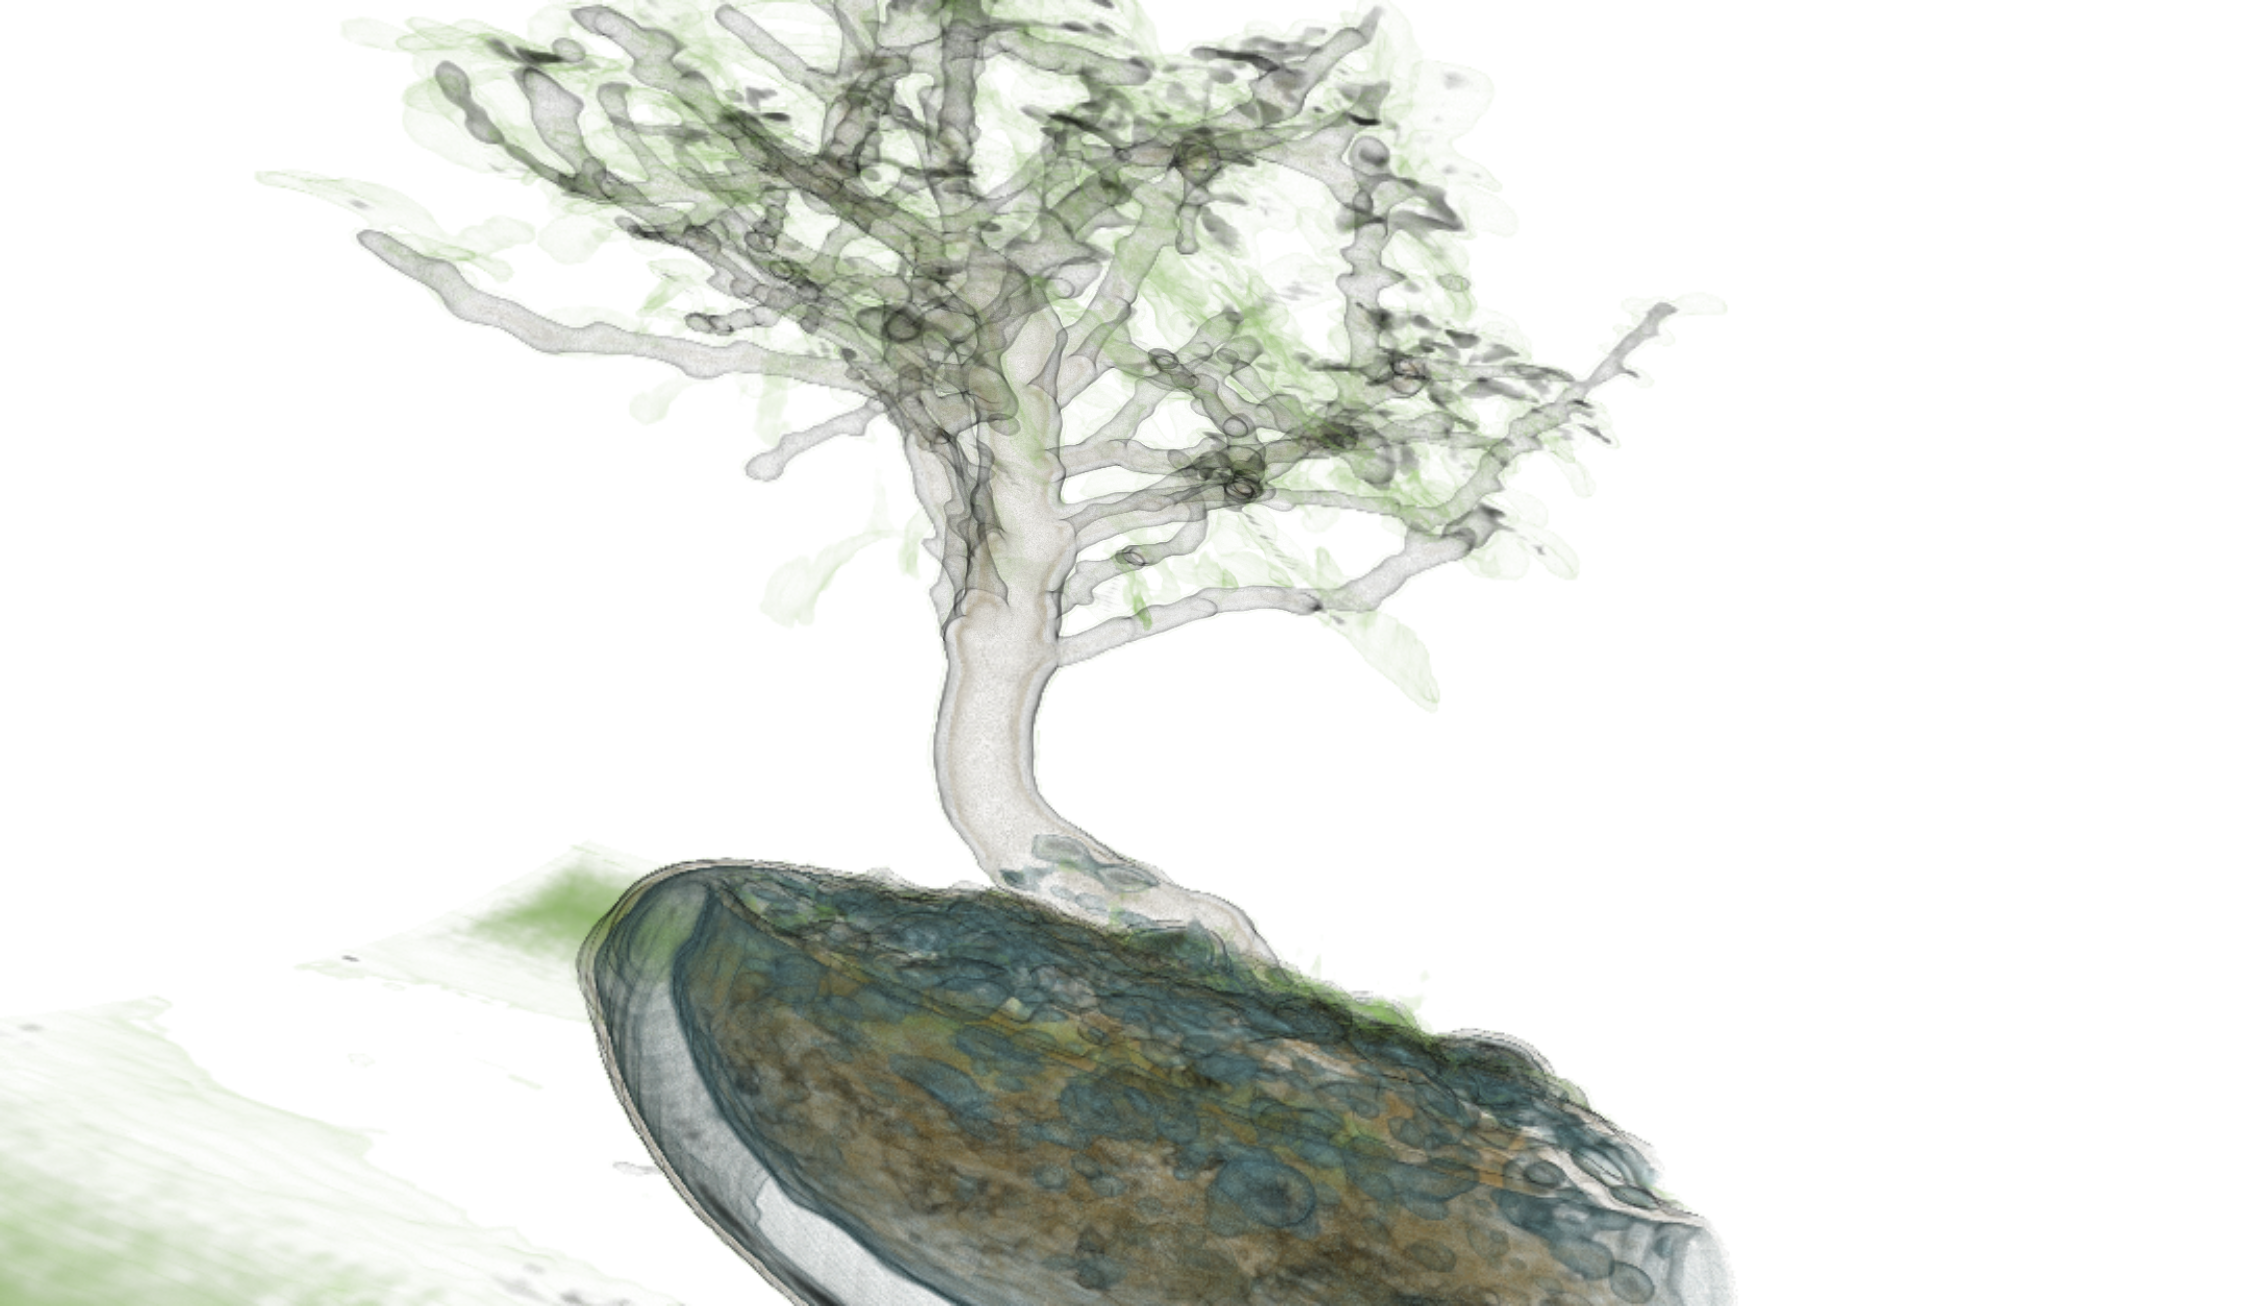
\includegraphics[width=1\textheight]{../../Neue_Messungen/Bonsai/mdc.png}
		\caption{Volumen Bonsai. Das Bild wurde mit dem \emph{MDC} Raycast berechnet. Ein kleiner Teil des Bildes, in Form eines Rechtecks, hat eine Bildabtastrate von $1,0$. Das restliche Bild hat nur eine Bildabtastrate von $0,5$. Die Strahlabtastrate beträgt für das ganze Bild $1.5$.}
		\label{fig::res::bon_mdc}
	\end{figure}
\end{landscape}

\begin{landscape}
	\begin{figure}
		\centering
		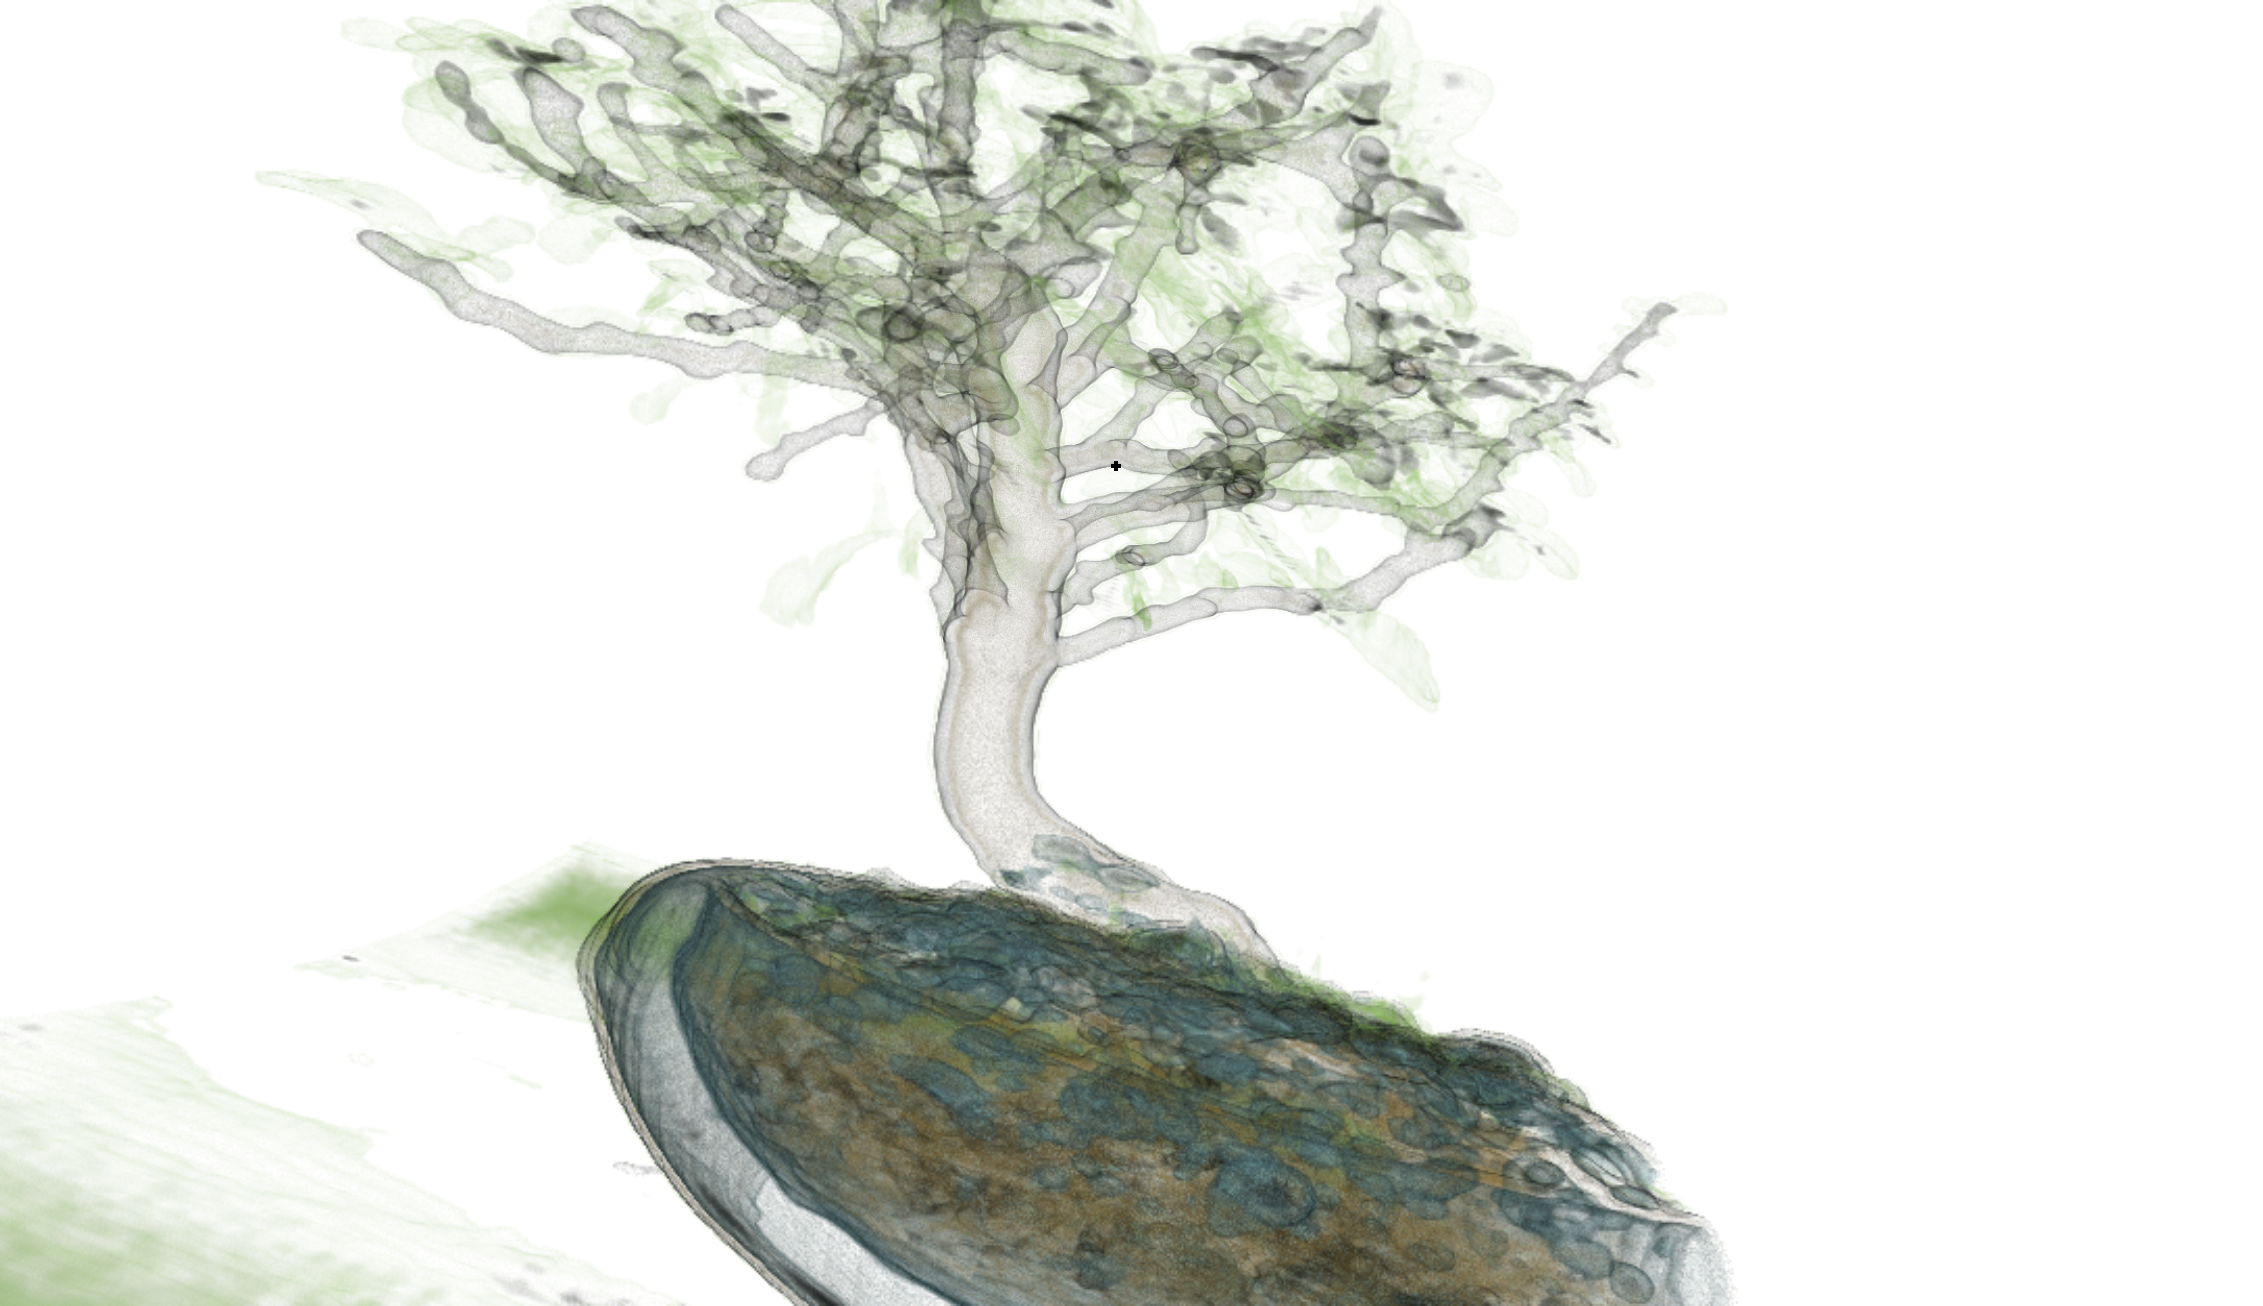
\includegraphics[width=1\textheight]{../../Neue_Messungen/Bonsai/mdc_ors.png}
		\caption{Volumen Bonsai. Das Bild wurde mit dem \emph{MDC} Raycast berechnet. Ein kleiner Teil des Bildes, in Form eines Rechtecks, hat eine Bildabtastrate von $1,0$. Das restliche Bild hat nur eine Bildabtastrate von $0,5$. Die Strahlabtastrate hat an der Mausposition einen Wert von $1,5$ und nimmt, abhängig von der Distanz zur Mausposition, bis zu einem Wert von $\frac{1,5}{4}$ ab.}
		\label{fig::res::bon_mdc_ors}
	\end{figure}
\end{landscape}

\iffalse
\begin{landscape}
	\begin{figure}[]
	\centering
	\begin{minipage}[t]{0.3\textheight}
		\centering
		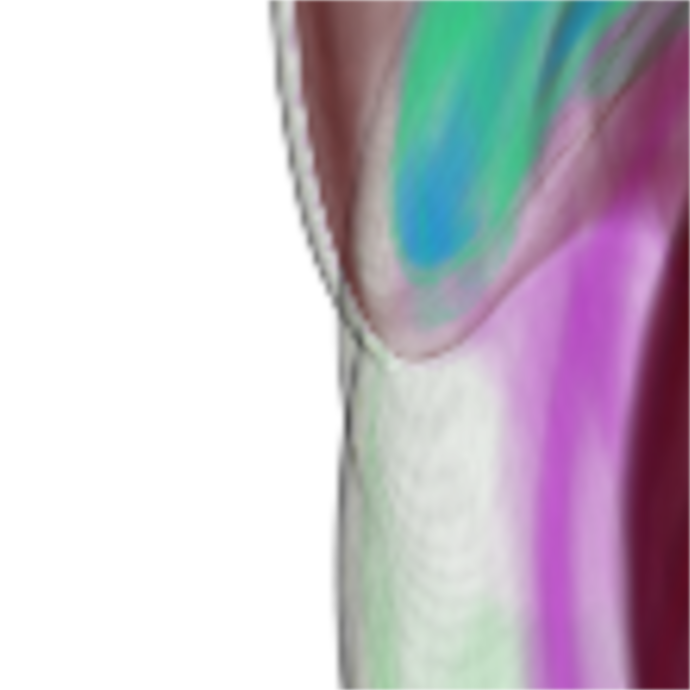
\includegraphics[width=1\textwidth]{../../Grafiken/results/picture_quality/supernova/comparison/MDC/mouse_away_mdc_cut.png}
		\caption*{Die Mausposition befindet sich außerhalb des Bildes, somit ist das Bild vollständig mit einer Bildabtastrate von $0,5$ berechnet worden.}
		\label{fig::res::sn_comp_mouse_away_mdc}
	\end{minipage}
	\hfill
	\begin{minipage}[t]{0.3\textheight}
		\centering
		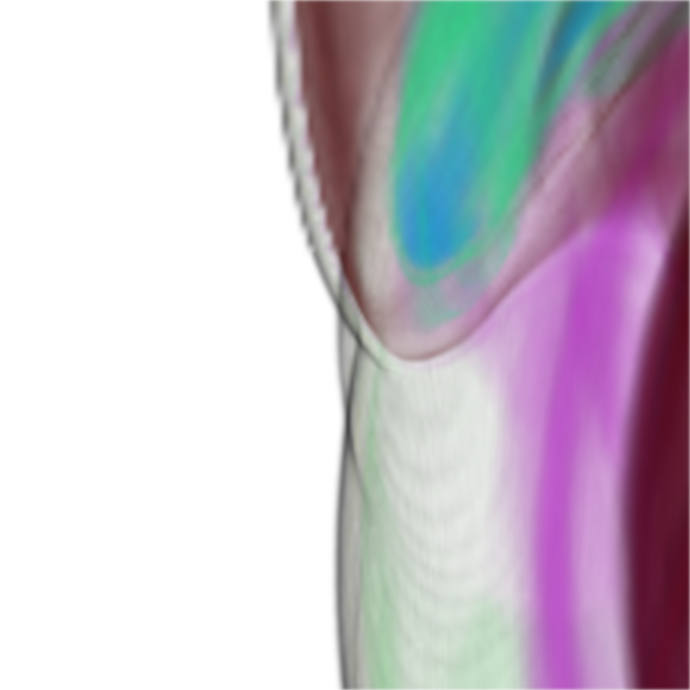
\includegraphics[width=1\textwidth]{../../Grafiken/results/picture_quality/supernova/comparison/MDC/mouse_half_on_mdc_cut.png}
		\caption*{Die Mausposition liegt so, dass das Rechteck nur einen Teil des Ausschnittes überdeckt.}
		\label{fig::res::sn_comp_mouse_half_on_mdc}
	\end{minipage}
	\hfill
	\begin{minipage}[t]{0.3\textheight}
		\centering
		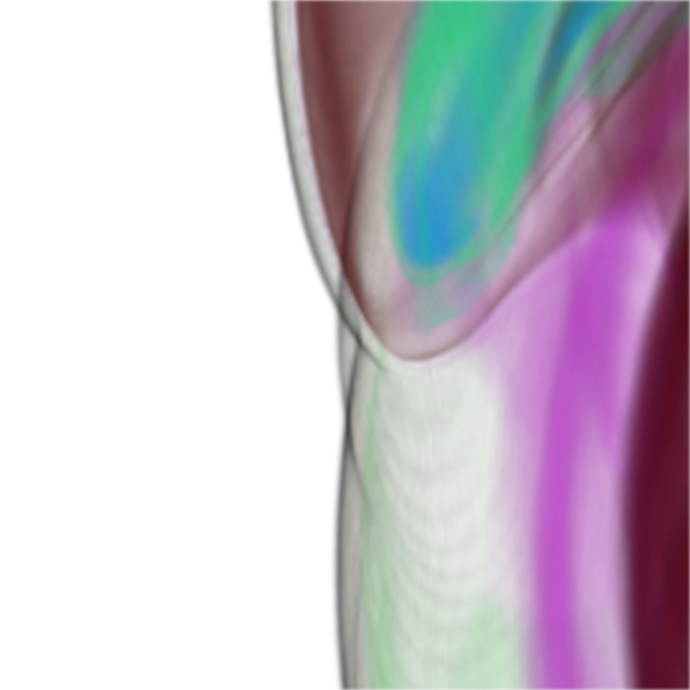
\includegraphics[width=1\textwidth]{../../Grafiken/results/picture_quality/supernova/comparison/MDC/mouse_on_mdc_cut.png}
		\caption*{Die Mausposition ist circa im Zentrum des Bildes. Der gesamte Ausschnitt liegt innerhalb dieses Rechtecks und hat eine Bildabtastrate von $1,0$.}
		\label{fig::res::sn_comp_mouse_on_mdc}
	\end{minipage}
	\caption{Ausschnitte dreier Berechnungen des Supernova Volumens mit der MDC Methode. Die Strahlabtastrate beträgt in der linken und rechten Abbildung für das ganze Bild $1.5$. Die Mausposition war bei den Berechnungen jeweils verschieden.}
	\end{figure}
\end{landscape}
\fi

\iffalse
\begin{landscape}
	\begin{figure}
		\centering
		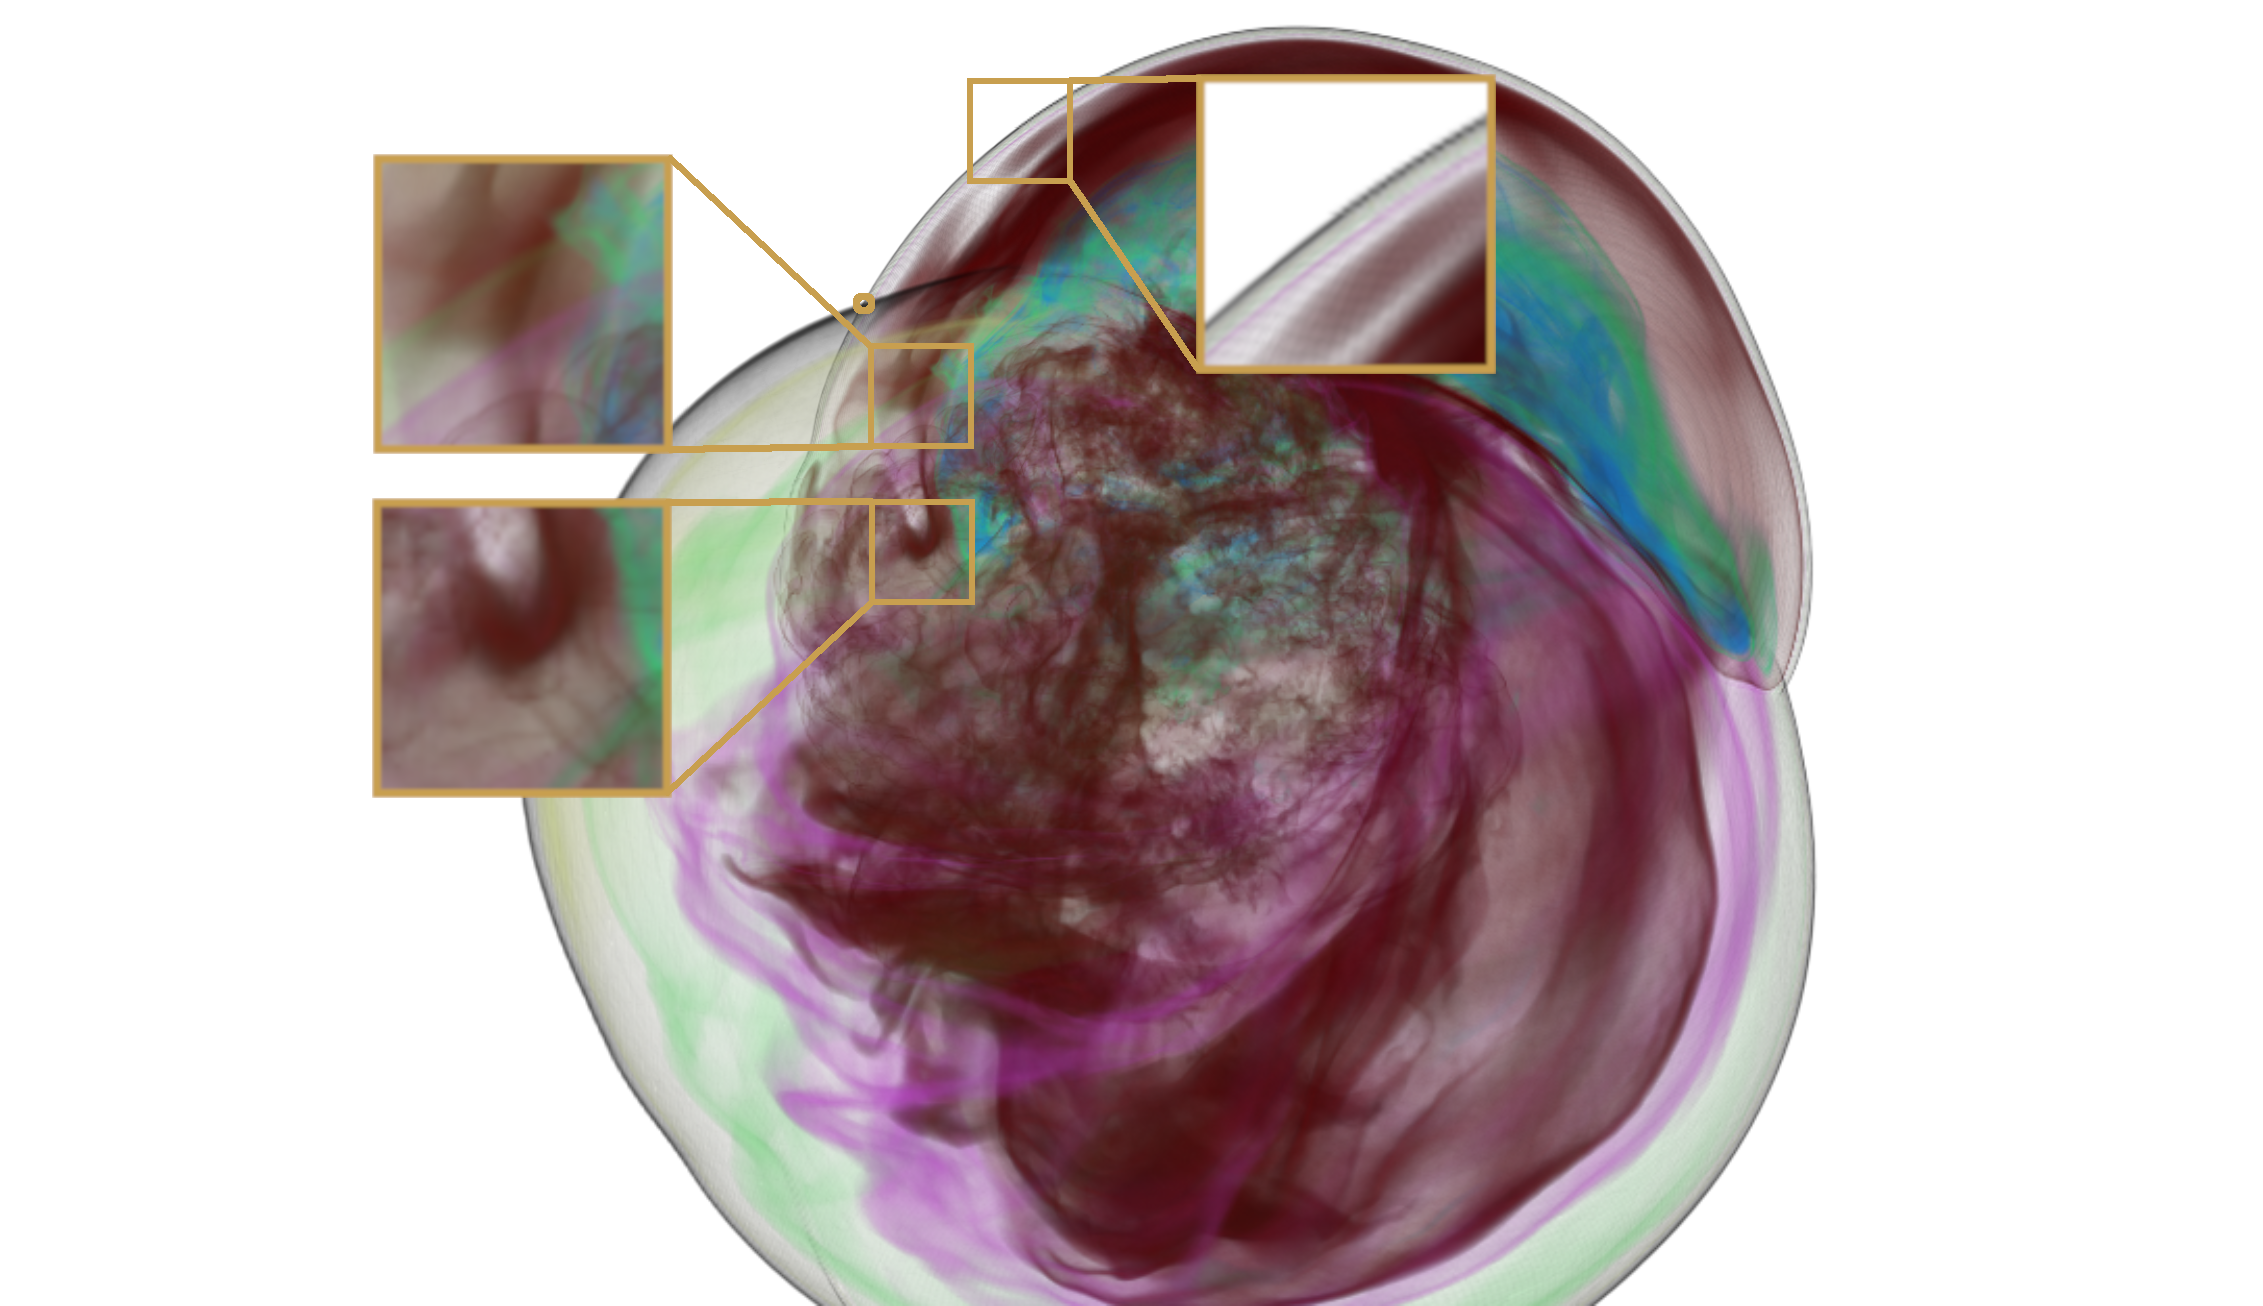
\includegraphics[width=\textheight]{../../Grafiken/results/picture_quality/supernova/MDC_img-0-96_ray-1-5_edited.png}
		\caption{Volumen Supernova mit \emph{MDC} Raycast berechnet mit vergrößerten Bildausschnitten.}
		\label{fig::res::sup_mdc}
	\end{figure}
\end{landscape}
\fi

\subsubsection{DDC Raycast}\label{ss::res::ddc}
Der \emph{DDC} Raycast ist das Ergebnis des Arbeitspakets aus dem Abschnitt \ref{ss::DDC}.
Abbildung \ref{fig::res::bon_ddc} zeigt das Volumen \emph{Bonsai}, welches mit dem \emph{DDC} Raycast erstellt wurde.
Das Bild wurde aus der selben Perspektive und mit der gleichen Transferfunktion berechnet, wie in den Abbildungen \ref{fig::res::bon_st} und \ref{fig::res::bon_mdc}.
Anders als beim Standard Raycast und \emph{MDC} Raycast, wo die Strahlabtastrate über das gesamte Bild hinweg gleich ist, nimmt beim \emph{DDC} Raycast die Strahlabtastrate Abhängig zur Distanz eines Strahls zur Maus- beziehungsweise Blickposition ab.
In einem kleinen Bereich um die Mausposition hat sie den maximalen Wert, der gleich dem Wert aus \emph{MDC} und dem Standard Raycast ist.
Die maximale Bildabtastrate ist $1$.
Diese nimmt in zwei Stufen nach außen hin ab.

Beim \emph{DDC} Raycast wurde nur ein Aufruf des Raycasts gestartet und die Work-Items und ihre entsprechenden Strahlen auf verschiedene Bildpunkte abgebildet.
Das gesamte Bild wurde in einem zweiten Kernel Aufruf interpoliert.
Innerhalb eines kleinen Bereichs in der Form einer Ellipse um den Blickpunkt herum hat das Bild eine Bildabtastrate von $1$, dass heißt jeder Pixel entspricht einem Farbwert der Auswertung eines Strahls.
Außerhalb von diesem Bereich aber innerhalb einer zweiten größeren und umschließenden Ellipse hat das Bild in x- und y-Richtung eine Bildabtastrate von $\frac{1}{2}$.
Das heißt, dass in x- und y-Richtung nur für jedes zweiten Pixel ein Strahl ausgewertet wird.
In dem äußersten Bereich beträgt die Bildabtastrate in x- und y-Richtung $\frac{1}{7}$.
Es wird also in jedem $7\times7$\,Pixel-Feld nur ein Strahl ausgewertet.

\todo{Mausposition einzeichnen.}

In Abbildung \ref{fig::res::bon_ddc} ist deutlich zu sehen, dass der Großteil des Bildes eine geringe Auflösung hat.
In dem am niedrigsten abgetasteten Bereich sind an den Konturen, insbesondere die der Äste, deutliche Merkmale der Unterabtastung zu sehen.
In Abbildung \ref{fig::res::bon_st} und \ref{fig::res::bon_mdc} verlaufen die Konturen der Äste noch diagonal und sind relativ weich gezeichnet, hier haben sie starke Treppeneffekte.

In dem mittleren Bereich ist die Bildqualität recht gut und die das Bild scharf zu erkennen.
Trotzdem hat das Bild hier nur ein Viertel der Auflösung.
Zwischen dem mittleren und inneren Bereich, welcher die normale Auflösung hat, ist kaum zu erkennen.

Dass die Strahlabtastrate mit zunehmender Entfernung zur Mausposition abnimmt, ist in Abbildung \ref{fig::res::bon_ddc} kaum zu erkennen.
Die reduzierte Auflösung verändert die Bildqualität im äußeren Bereich so stark, dass die reduzierte Strahlabtastrate nicht auffällt.

Bei aktivem Eyetracking wird anstelle der Mausposition die aktuelle Blickposition verwendet.
Der Fokus liegt bei aktivem Eyetracking nun im Zentrum des inneren Bereichs.
Der innere Bereich ist groß genug, so dass der Abfall der Bildabtastrate zum mittleren Bereich nicht auffällt.
Zusammen ergeben der innere und mittlere Bereich den Teil des Bildes, in welchem das Bild scharf zu sehen ist.
Anders als in Abbildung \ref{fig::res::bon_mdc}, ist es in Abbildung \ref{fig::res::bon_ddc} auch wenn der innere und mittlere Bereich auf den Blickpunkt zentriert sind, auffallend, dass der äußere Bereich mit einer deutlich niedrigeren Bildabtastrate berechnet wurde.
Die grundlegenden Konturen des Bildes können aber im äußeren Bereich noch erkannt werden wodurch das Identifizieren von interessanten Objekten immer noch möglich ist.
Der äußere Bereich ist von dem Zentrum der Blickpunktes so weit entfernt, dass um mehr Informationen über Objekte im äußeren Bereich erhalten zu können, unabhängig von der Bildabtastrate des äußeren Bereichs eine Augenbewegung notwendig ist.
Die Sehschärfe ist bei dieser Distanz zur Fovea zu schwach, um dies ohne den Blickpunkt zu bewegen, zu erreichen.

% Abbildung \ref{fig::res::sup_ddc} zeigt das selbe Volumen wie in Abbildung \ref{fig::res::sup_st} und \ref{fig::res::sup_mdc}. ; Direkter Vergleich
% Bildausschnitte der Übergänge zwischen den Bereichen sind hier zur Verdeutlichung hervorgehoben und vergrößert.
% Der vergrößerte Bildausschnitt rechts oben zeigt den Übergang zwischen dem mittleren und dem inneren Bereich.
% Oben links ist der vergrößerte Übergang zwischen dem inneren und dem mittleren Bereich zu sehen.
% Der Bildausschnitt unten links ist etwas größer und umfasst den Übergang von dem inneren zum mittleren und vom mittleren zum äußeren Bereich.

\begin{landscape}
	\begin{figure}
		\centering
		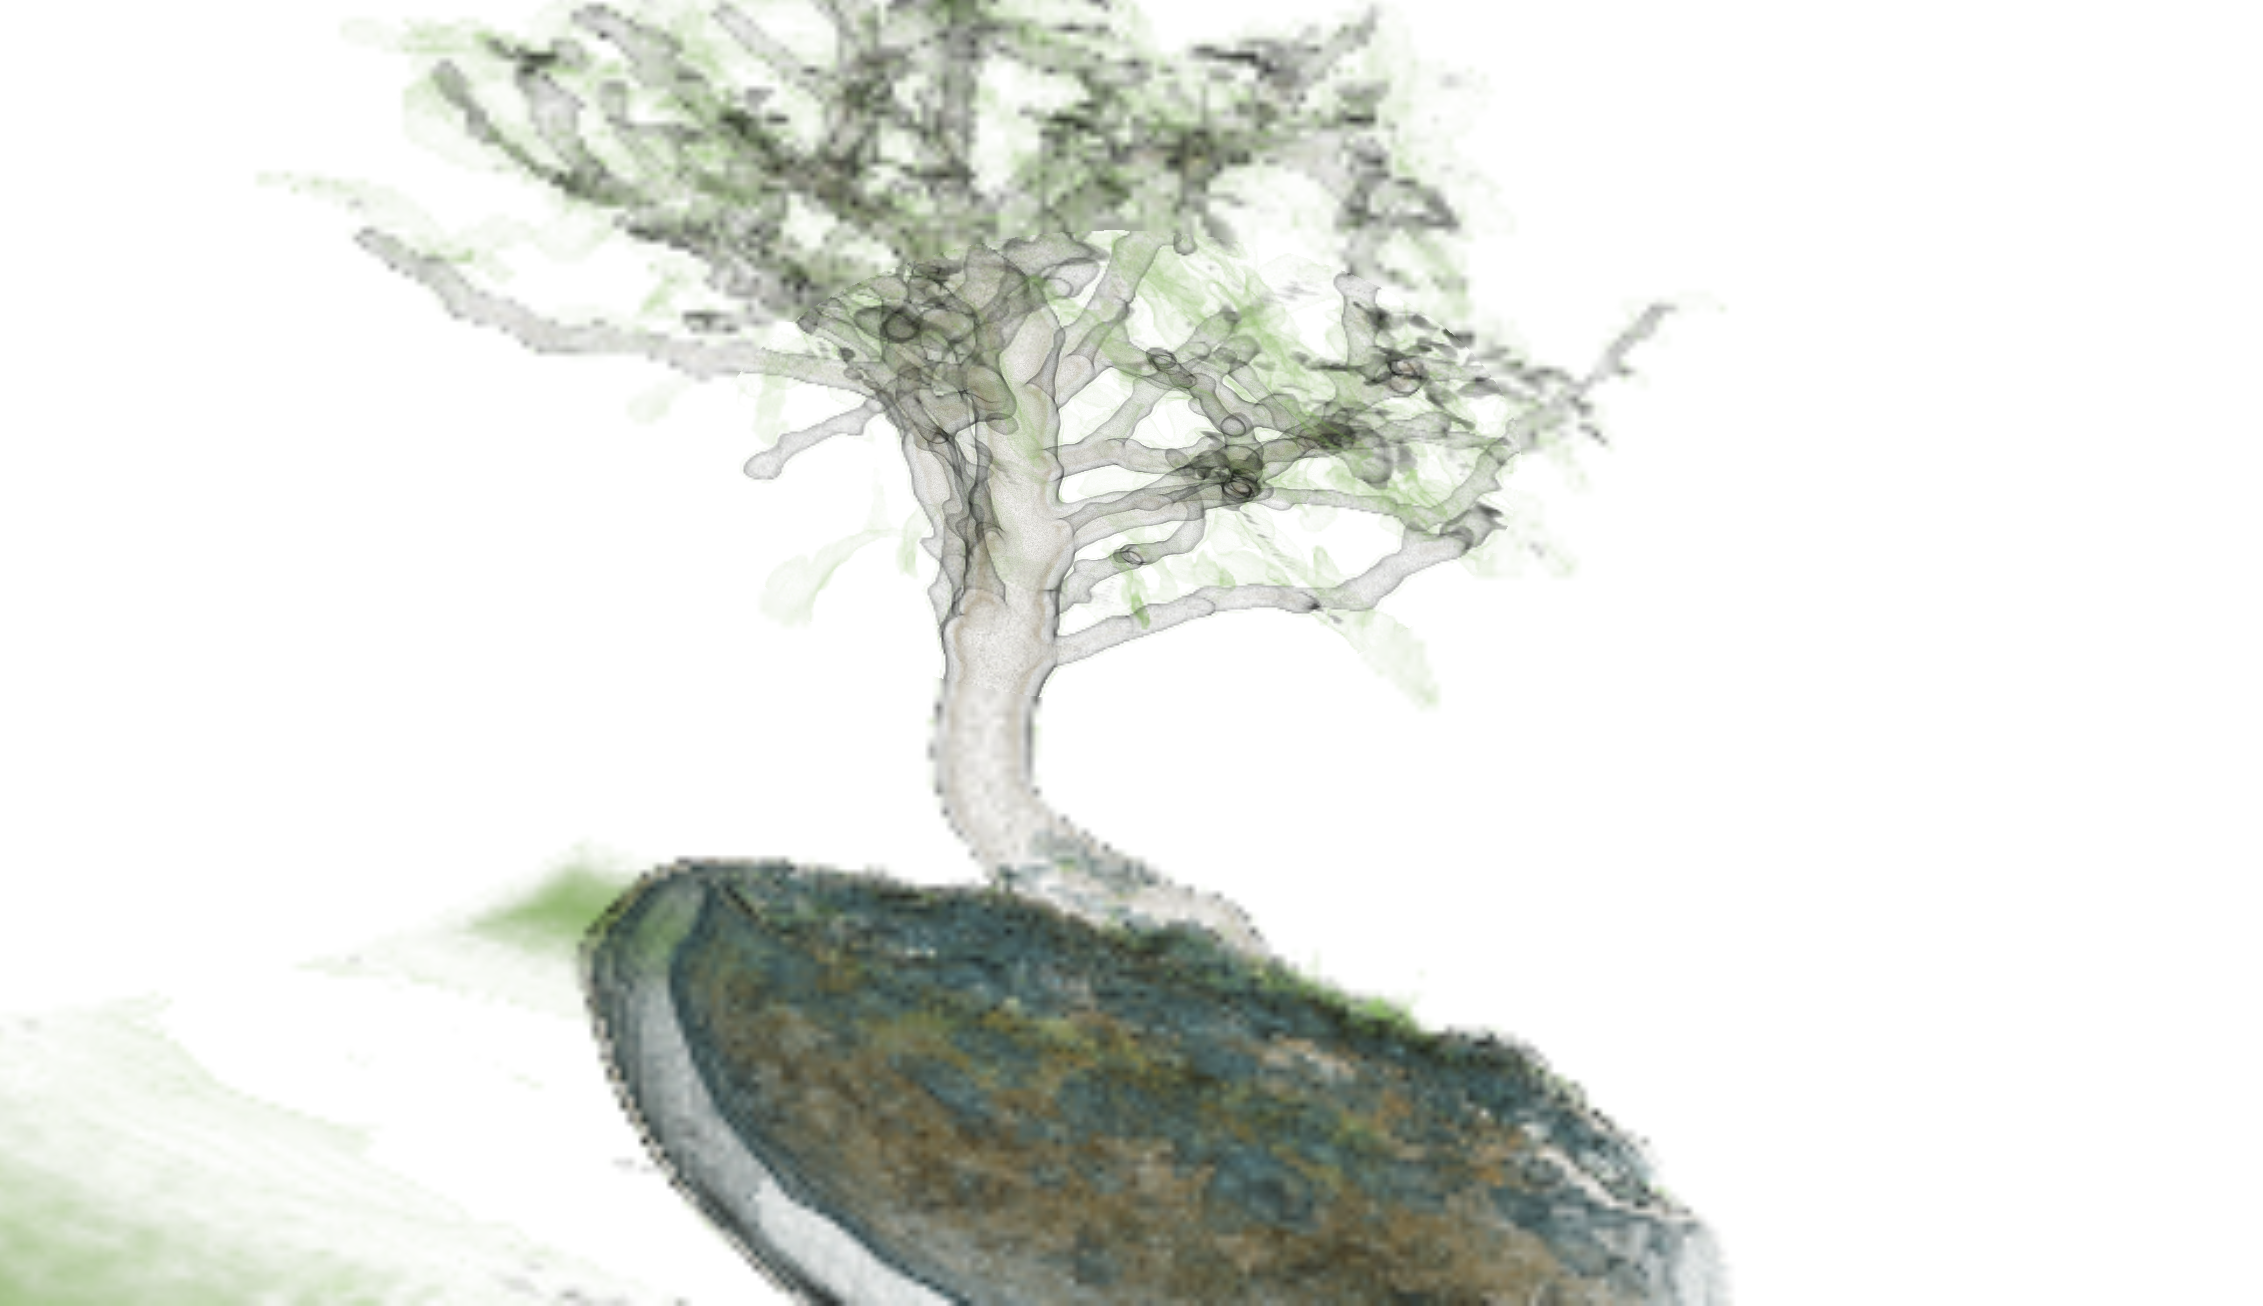
\includegraphics[width=1\textheight]{../../Neue_Messungen/Bonsai/ddc.png}
		\caption{Volumen Bonsai mit \emph{DDC} Raycast berechnet. Die Bildabtastrate nimmt nach außen hin in zwei Schritten ab. An der Mausposition hat sie den höchsten Wert von $1,0$. Etwas weiter außen einen Wert von $0,5$ und noch weiter außen hat sie den niedrigsten Wert von $\frac{1}{7}$. Die Strahlabtastrate beträgt für das ganze Bild $1.5$.}
		\label{fig::res::bon_ddc}
	\end{figure}
\end{landscape}

\begin{landscape}
	\begin{figure}
		\centering
		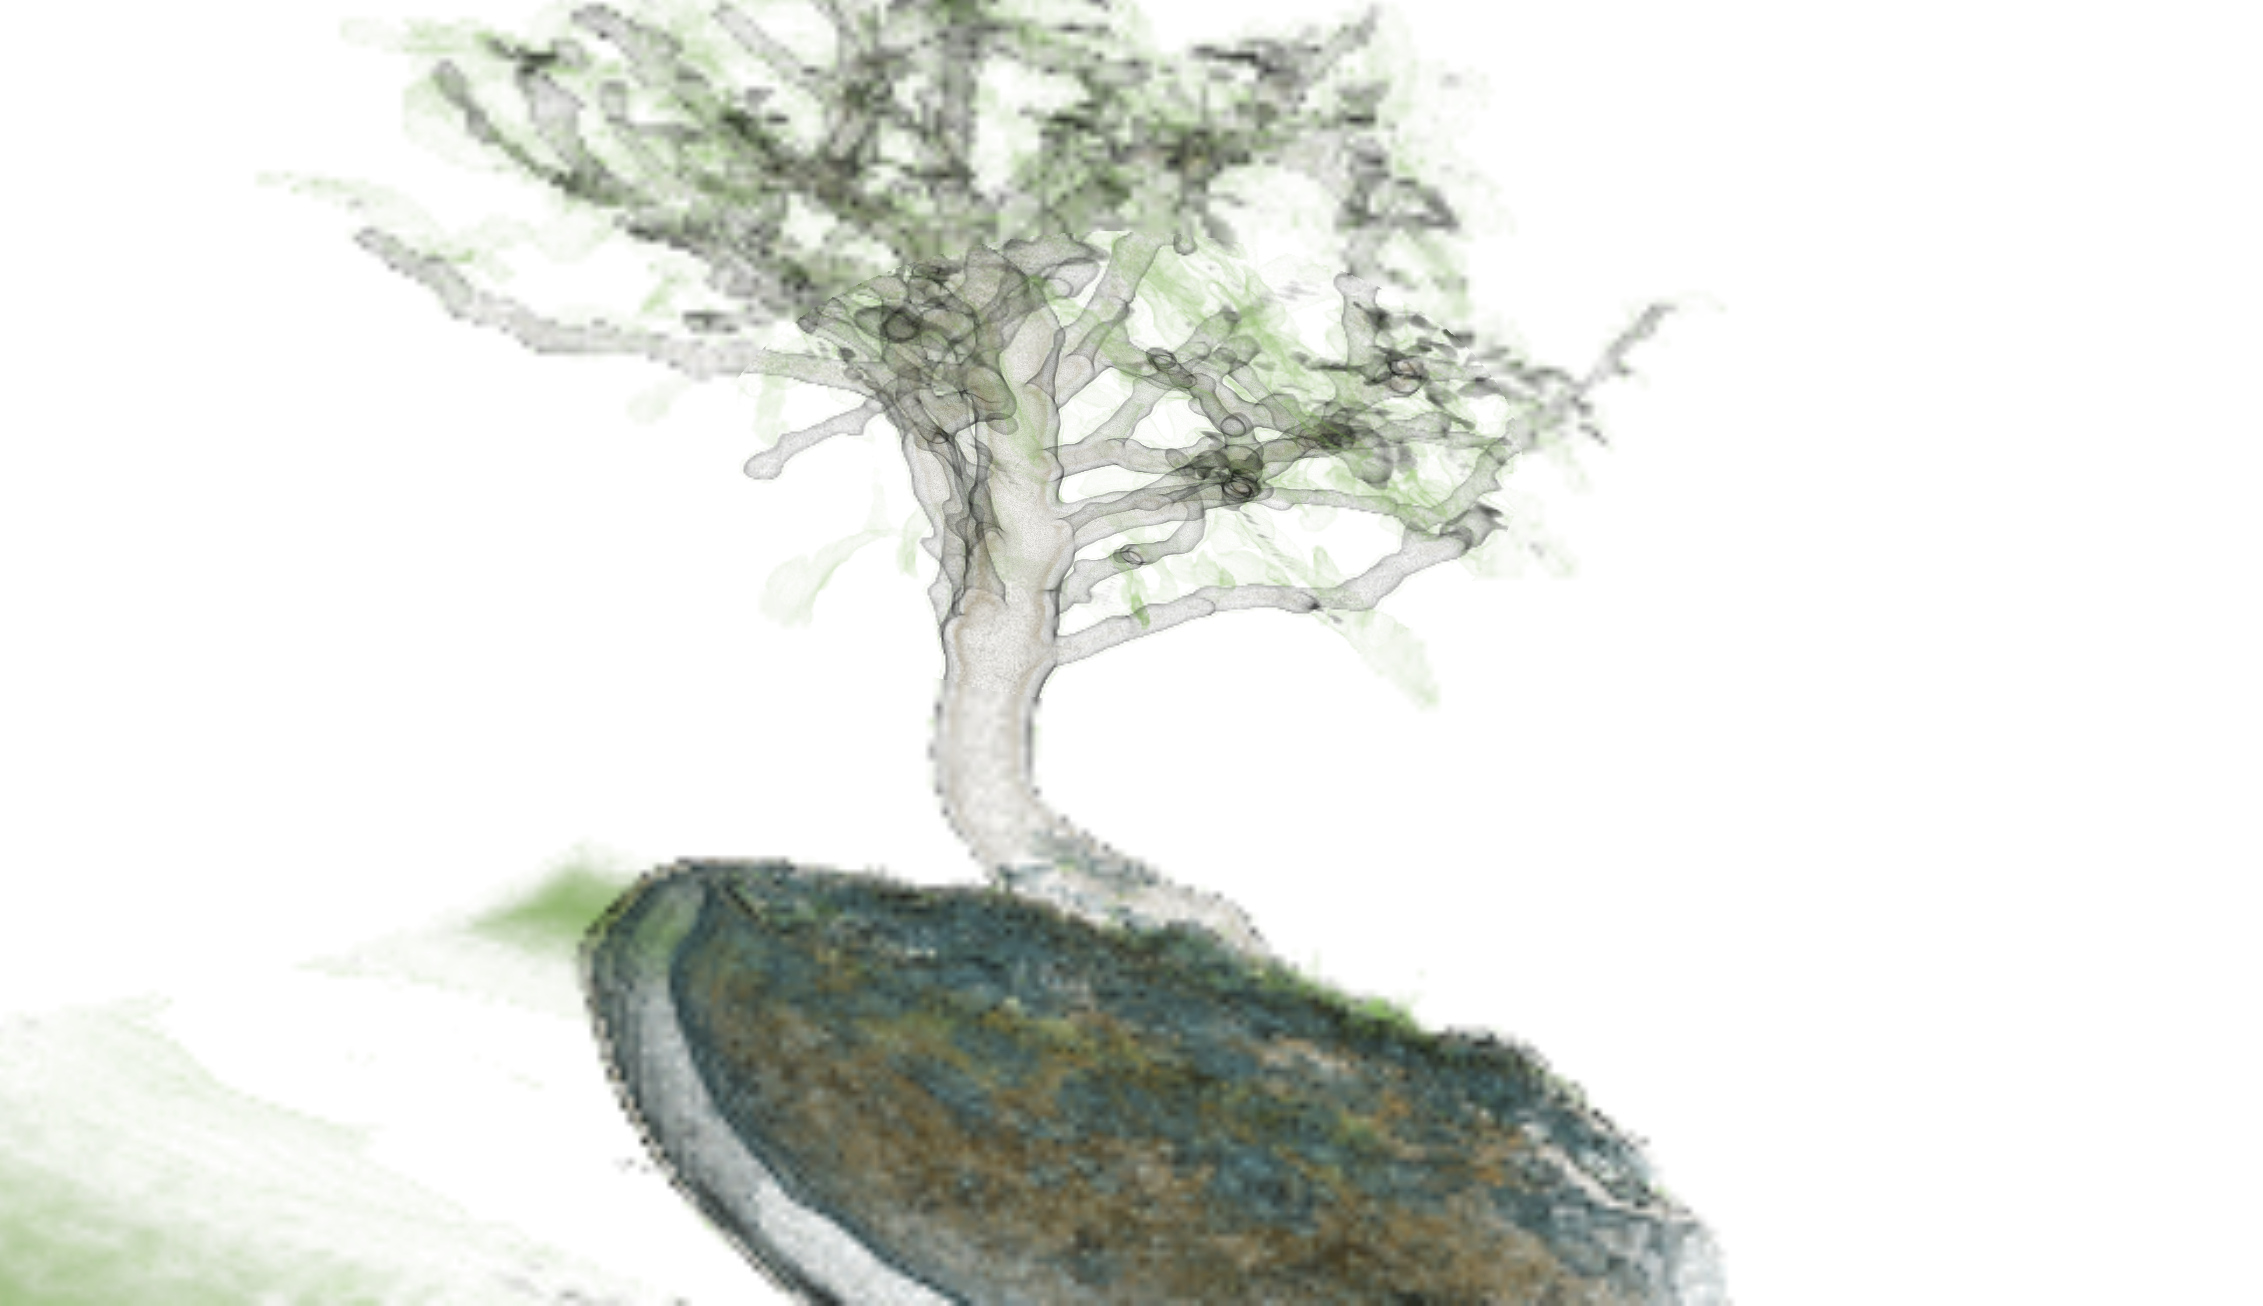
\includegraphics[width=1\textheight]{../../Neue_Messungen/Bonsai/ddc_ors.png}
		\caption{Volumen Bonsai mit \emph{DDC} Raycast berechnet. Die Bildabtastrate nimmt nach außen hin in zwei Schritten ab. An der Mausposition hat sie den höchsten Wert von $1,0$, weiter außen einen Wert von $0,5$, dann einen Wert von $\frac{1}{7}$. Die Strahlabtastrate hat an der Mausposition einen Wert von $1,5$ und nimmt, abhängig von der Distanz zur Mausposition, bis zu einem Wert von $\frac{1,5}{4}$ ab.}
		\label{fig::res::bon_ddc_ors}
	\end{figure}
\end{landscape}

\subsubsection*{Direkter Vergleich}

\begin{landscape}
	\begin{figure}
		\centering
		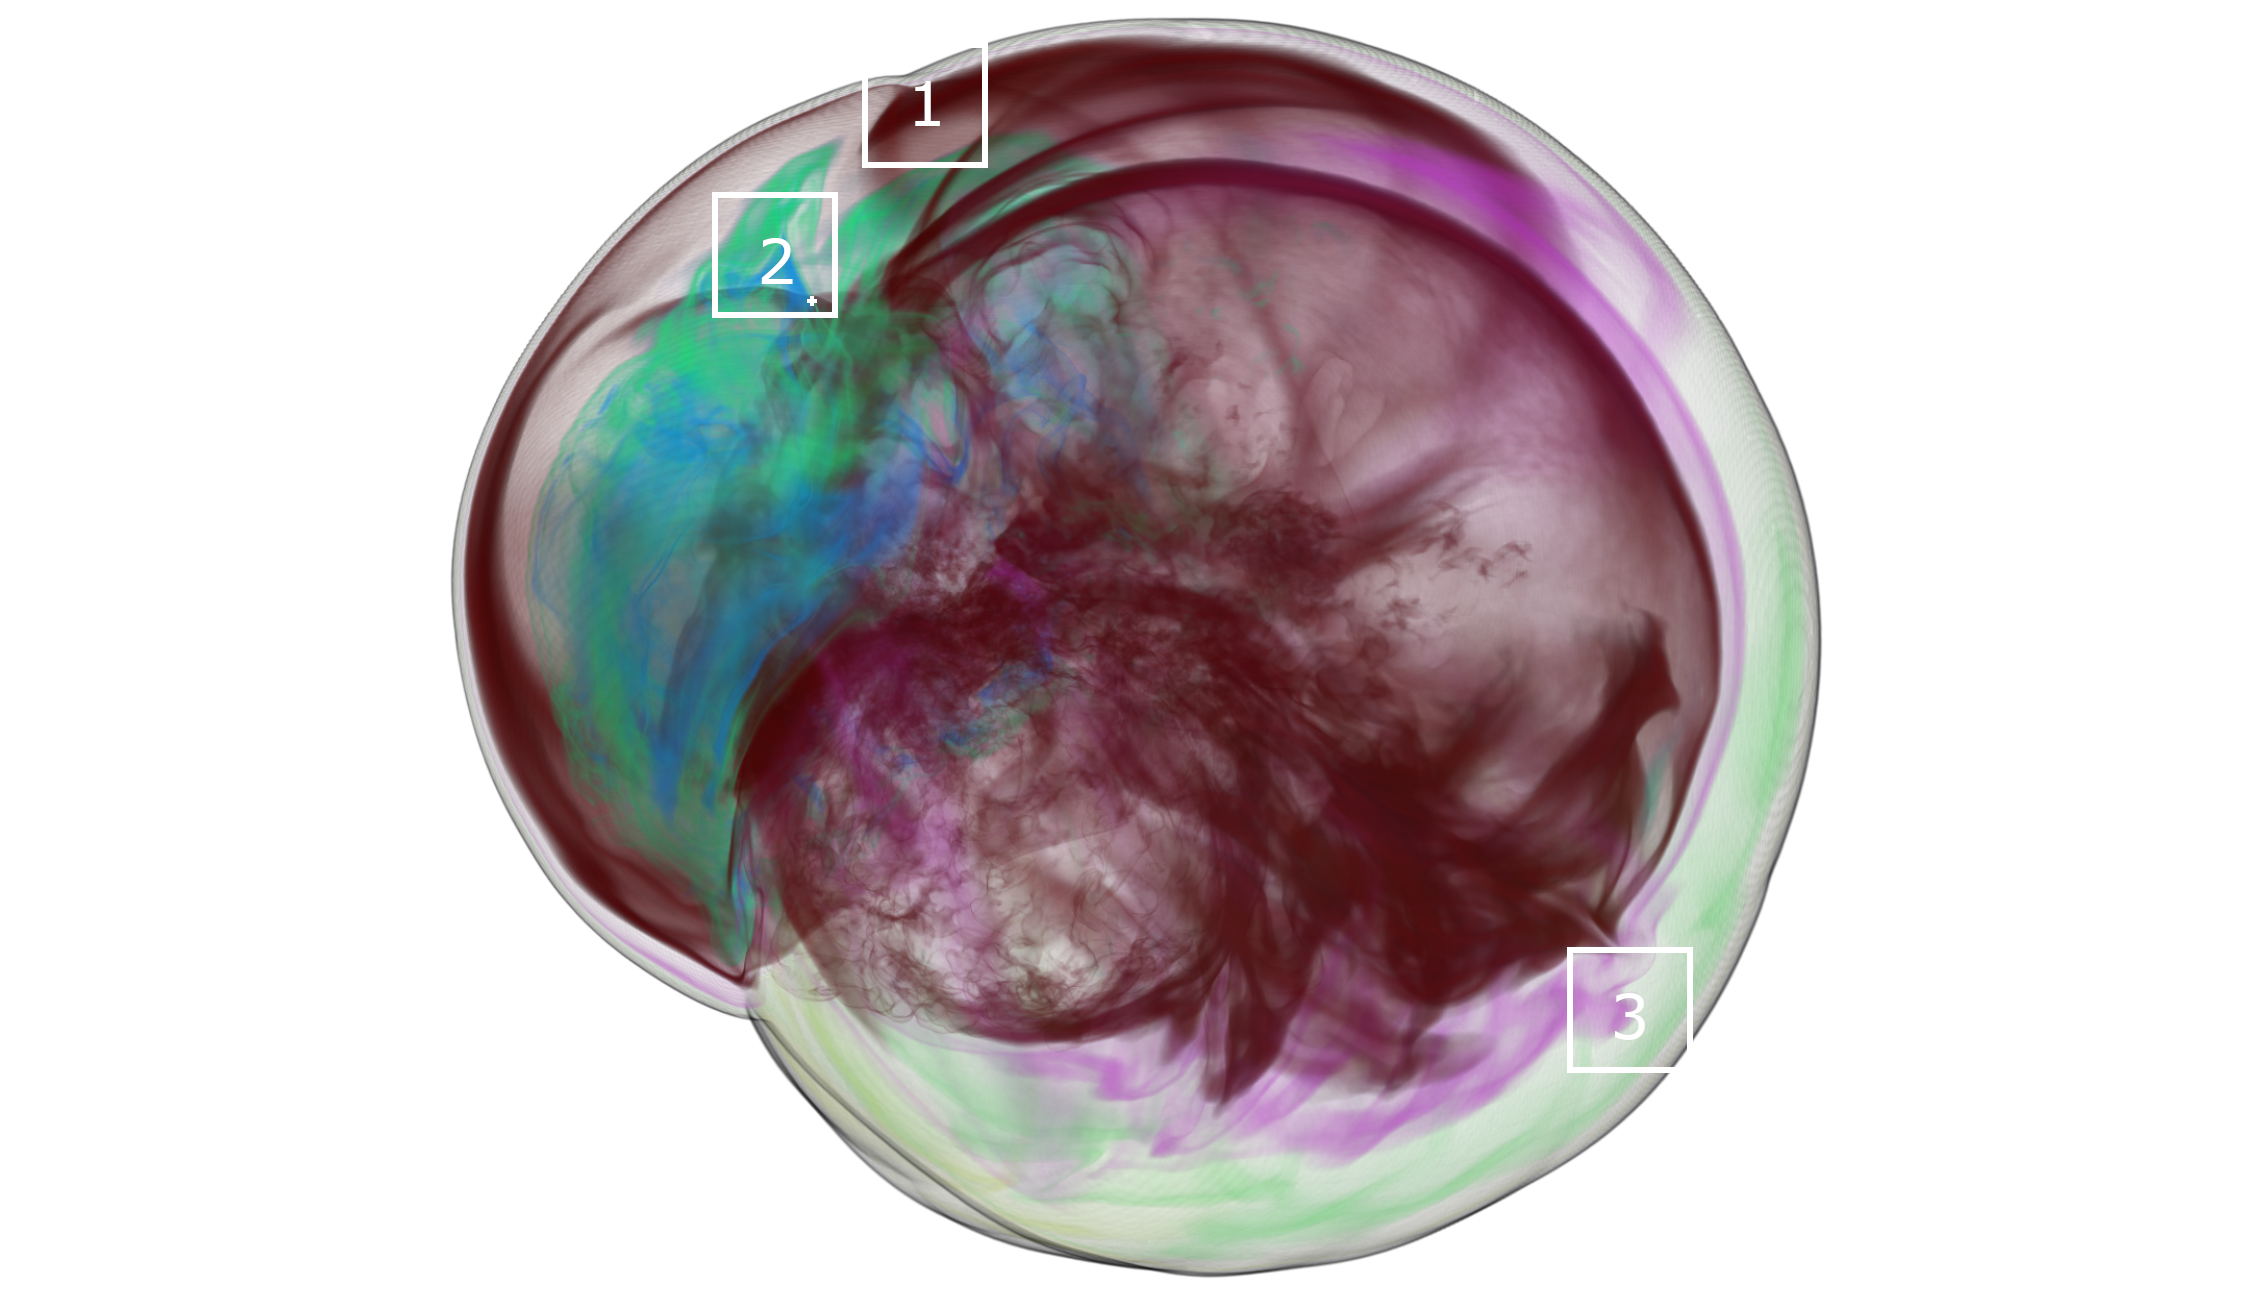
\includegraphics[width=1\textheight]{../../Neue_Messungen/Supernova/cut/st/st_123.png}
		\caption{Ein Zeitschritt der Supernova mit dem Standard Raycast berechnet. Die Bildabtastrate beträgt für das ganze Bild $1$. Die Strahlabtastrate beträgt für das ganze Bild $1,5$. die Mausposition und drei nummerierte Quadrate sind eingezeichnet, die Positionen der Quadrate werden im folgenden Vergleich verwendet.}
		\label{fig::res::sn_comp_st_123}
	\end{figure}
\end{landscape}

\begin{figure}[]
	\centering
	\begin{minipage}[t]{0.3\textwidth}
		\centering
		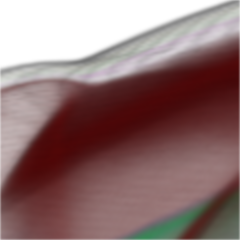
\includegraphics[width=1\textwidth]{../../Neue_Messungen/Supernova/cut/st/st_1.png}
		% \caption*{Quadrat 1 vergrößert dargestellt.}
		% \label{fig::res::sn_comp_st_1}
	\end{minipage}
	\hfill
	\begin{minipage}[t]{0.3\textwidth}
		\centering
		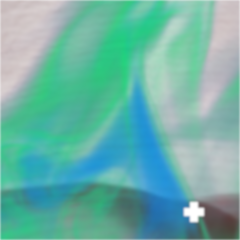
\includegraphics[width=1\textwidth]{../../Neue_Messungen/Supernova/cut/st/st_2.png}
		% \caption*{Quadrat 2 vergrößert dargestellt.}
		% \label{fig::res::sn_comp_st_2}
	\end{minipage}
	\hfill
	\begin{minipage}[t]{0.3\textwidth}
		\centering
		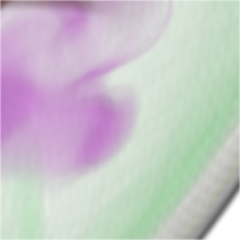
\includegraphics[width=1\textwidth]{../../Neue_Messungen/Supernova/cut/st/st_3.png}
		% \caption*{Quadrat 3 vergrößert dargestellt.}
		% \label{fig::res::sn_comp_st_3}
	\end{minipage}
	\caption{Supernova mit Standard Raycast und ohne variierter Strahlabtastrate berechnet.}
	\label{fig::res::sn_comp_st}
\end{figure}

\begin{figure}[]
	\centering
	\begin{minipage}[t]{0.3\textwidth}
		\centering
		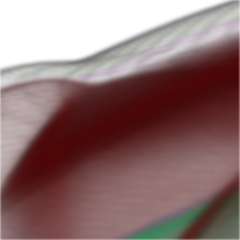
\includegraphics[width=1\textwidth]{../../Neue_Messungen/Supernova/cut/st_ors/st_ors_1.png}
		% \caption*{Quadrat 1 vergrößert dargestellt.}
		% \label{fig::res::sn_comp_st_ors_1}
	\end{minipage}
	\hfill
	\begin{minipage}[t]{0.3\textwidth}
		\centering
		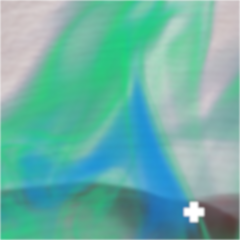
\includegraphics[width=1\textwidth]{../../Neue_Messungen/Supernova/cut/st_ors/st_ors_2.png}
		% \caption*{Quadrat 2 vergrößert dargestellt.}
		% \label{fig::res::sn_comp_st_ors_2}
	\end{minipage}
	\hfill
	\begin{minipage}[t]{0.3\textwidth}
		\centering
		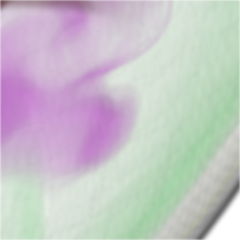
\includegraphics[width=1\textwidth]{../../Neue_Messungen/Supernova/cut/st_ors/st_ors_3.png}
		% \caption*{Quadrat 3 vergrößert dargestellt.}
		% \label{fig::res::sn_comp_st_ors_3}
	\end{minipage}
	\caption{Supernova mit Standard Raycast und variierter Strahlabtastrate berechnet.}
	\label{fig::res::sn_comp_st_ors}
\end{figure}

\begin{figure}[]
	\centering
	\begin{minipage}[t]{0.3\textwidth}
		\centering
		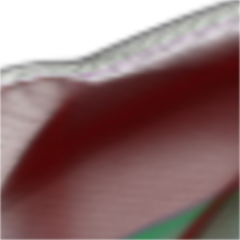
\includegraphics[width=1\textwidth]{../../Neue_Messungen/Supernova/cut/mdc/mdc_1.png}
		% \caption*{Quadrat 1 vergrößert dargestellt.}
		% \label{fig::res::sn_comp_mdc_1}
	\end{minipage}
	\hfill
	\begin{minipage}[t]{0.3\textwidth}
		\centering
		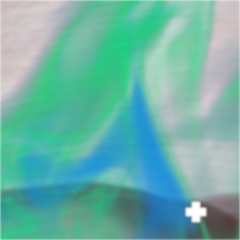
\includegraphics[width=1\textwidth]{../../Neue_Messungen/Supernova/cut/mdc/mdc_2.png}
		% \caption*{Quadrat 2 vergrößert dargestellt.}
		% \label{fig::res::sn_comp_mdc_2}
	\end{minipage}
	\hfill
	\begin{minipage}[t]{0.3\textwidth}
		\centering
		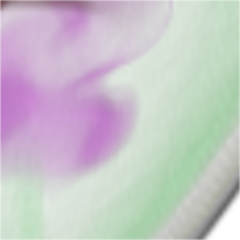
\includegraphics[width=1\textwidth]{../../Neue_Messungen/Supernova/cut/mdc/mdc_3.png}
		% \caption*{Quadrat 3 vergrößert dargestellt.}
		% \label{fig::res::sn_comp_mdc_3}
	\end{minipage}
	\caption{Supernova mit MDC Raycast und ohne variierter Strahlabtastrate berechnet.}
	\label{fig::res::sn_comp_mdc}
\end{figure}

\begin{figure}[]
	\centering
	\begin{minipage}[t]{0.3\textwidth}
		\centering
		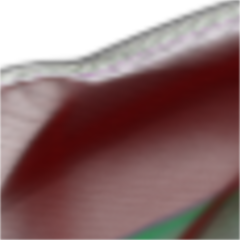
\includegraphics[width=1\textwidth]{../../Neue_Messungen/Supernova/cut/mdc_ors/mdc_ors_1.png}
		% \caption*{Quadrat 1 vergrößert dargestellt.}
		% \label{fig::res::sn_comp_mdc_ors_1}
	\end{minipage}
	\hfill
	\begin{minipage}[t]{0.3\textwidth}
		\centering
		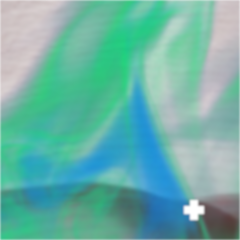
\includegraphics[width=1\textwidth]{../../Neue_Messungen/Supernova/cut/mdc_ors/mdc_ors_2.png}
		% \caption*{Quadrat 2 vergrößert dargestellt.}
		% \label{fig::res::sn_comp_mdc_ors_2}
	\end{minipage}
	\hfill
	\begin{minipage}[t]{0.3\textwidth}
		\centering
		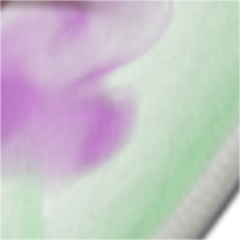
\includegraphics[width=1\textwidth]{../../Neue_Messungen/Supernova/cut/mdc_ors/mdc_ors_3.png}
		% \caption*{Quadrat 3 vergrößert dargestellt.}
		% \label{fig::res::sn_comp_mdc_ors_3}
	\end{minipage}
	\caption{Supernova mit MDC Raycast und variierter Strahlabtastrate berechnet.}
	\label{fig::res::sn_comp_mdc_ors}
\end{figure}

\begin{figure}[]
	\centering
	\begin{minipage}[t]{0.3\textwidth}
		\centering
		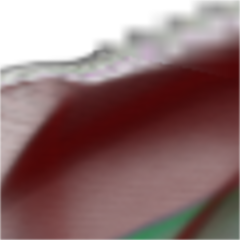
\includegraphics[width=1\textwidth]{../../Neue_Messungen/Supernova/cut/ddc/ddc_1.png}
		% \caption*{Quadrat 1 vergrößert dargestellt.}
		% \label{fig::res::sn_comp_ddc_1}
	\end{minipage}
	\hfill
	\begin{minipage}[t]{0.3\textwidth}
		\centering
		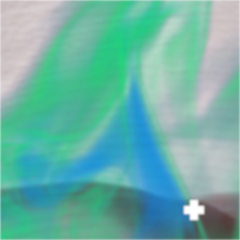
\includegraphics[width=1\textwidth]{../../Neue_Messungen/Supernova/cut/ddc/ddc_2.png}
		% \caption*{Quadrat 2 vergrößert dargestellt.}
		% \label{fig::res::sn_comp_ddc_2}
	\end{minipage}
	\hfill
	\begin{minipage}[t]{0.3\textwidth}
		\centering
		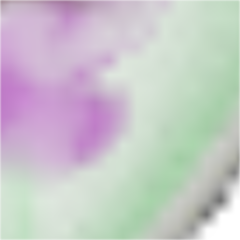
\includegraphics[width=1\textwidth]{../../Neue_Messungen/Supernova/cut/ddc/ddc_3.png}
		% \caption*{Quadrat 3 vergrößert dargestellt.}
		% \label{fig::res::sn_comp_ddc_3}
	\end{minipage}
	\caption{Supernova mit DDC Raycast und ohne variierter Strahlabtastrate berechnet.}
	\label{fig::res::sn_comp_ddc}
\end{figure}

\begin{figure}[]
	\centering
	\begin{minipage}[t]{0.3\textwidth}
		\centering
		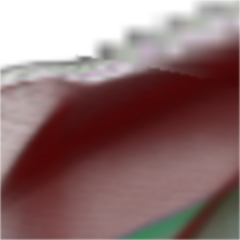
\includegraphics[width=1\textwidth]{../../Neue_Messungen/Supernova/cut/ddc_ors/ddc_ors_1.png}
		% \caption*{Quadrat 1 vergrößert dargestellt.}
		% \label{fig::res::sn_comp_ddc_ors_1}
	\end{minipage}
	\hfill
	\begin{minipage}[t]{0.3\textwidth}
		\centering
		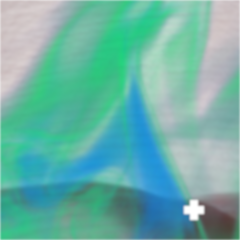
\includegraphics[width=1\textwidth]{../../Neue_Messungen/Supernova/cut/ddc_ors/ddc_ors_2.png}
		% \caption*{Quadrat 2 vergrößert dargestellt.}
		% \label{fig::res::sn_comp_ddc_ors_2}
	\end{minipage}
	\hfill
	\begin{minipage}[t]{0.3\textwidth}
		\centering
		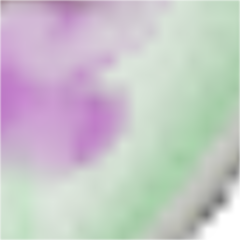
\includegraphics[width=1\textwidth]{../../Neue_Messungen/Supernova/cut/ddc_ors/ddc_ors_3.png}
		% \caption*{Quadrat 3 vergrößert dargestellt.}
		% \label{fig::res::sn_comp_ddc_ors_3}
	\end{minipage}
	\caption{Supernova mit DDC Raycast und ohne variierter Strahlabtastrate berechnet.}
	\label{fig::res::sn_comp_ddc_ors}
\end{figure}

\clearpage

\subsection{Performanz}
Für die Messung der Performanz der Implementierungen wurden zwei Messwerte bei einer Berechnung eines Bildes genommen.
Die Ausführungszeit des Kernels innerhalb einer Ausführung der \emph{paintGL()}-Methode und die Ausführungszeit der \emph{paintGL()}-Methode selbst.
Dies wurde deshalb so gewählt, da die Implementierungen nicht ausschließlich innerhalb des Kernels durchgeführt wurden, sondern auch außerhalb der Kernelaufrufe Programmcode geschrieben wurde und der Start einer Kernelausführung sowie die synchronisierte Beendigung eine gewisse Zeit brauchen.
Die Ausführungszeit der \emph{paintGL()}-Methode ist letztendlich der Wert, welcher die reale spürbare Performanz für den Nutzer angibt.

Für die Messungen der Performanz wurde kein Eyetracking verwendet, da dies lediglich die Mausposition mit der Blickposition ersetzt und keinen Einfluss auf die Ausführungszeit des Kernels und nur einen konstanten Einfluss auf die Ausführungszeit der \emph{paintGL()}-Methode hat.
Außerdem wurde in Arbeitspaket \ref{sec::workpacks::evm} gefordert, dass eine Messung reproduzierbar sein soll.
Die Verwendung eines Eyetrackers würde es fast unmöglich machen, die selben Blickpunkte in einem gewissen Zeitraum zu fokussieren.

Für die Messergebnisse selbst wurde ein spiegelverkehrtes S mit dem Mauszeiger auf einem Bild nachgefahren und dabei die Mauspositionen abgespeichert.
Es wurden anschließend verschiedene Volumendaten mit jeweils drei verschiedenen Transferfunktionen für die drei verschiedenen Implementierungen, den Standard-, \emph{MDC}- und \emph{DDC}-Raycast, für die Messungen verwendet.
Bei jeder dieser Messung wurde dabei für jede der Mauspositionen des gespeicherten Mausverlaufs ein Bild berechnet und zu dieser Berechnung die Mausposition, Ausführungszeit des Kernels und Ausführungszeit der \emph{paintGL()}-Methode gespeichert.

Die Hardware des Computers, mit welchem die Messungen durchgeführt wurden, besteht aus einem \emph{Intel Core i5 4670k bei $3,40$\,GHz} CPU und einer \emph{GIGABYTE AMD Radeon (TM) R9 390 Series} GPU.
Die Auflösung der zu berechnenden Bilder betrug $2263\times1306$\,Pixel.

Im folgenden werden verschiedene Messungen vorgestellt.
Aus den gemessenen Ausführungszeiten des Kernels wurden Heatmaps für das jeweils zugrundeliegende Bild erstellt.
Da die Differenz zwischen Ausführungszeit des Kernels und der Ausführungszeit der \emph{paintGL()}-Methode unabhängig von dem zu berechnenden Volumen und der verwendeten Transferfunktion ist, wurde diese nicht für die Erstellung der Heatmaps einbezogen.
Die Ausführungszeiten insbesondere der \emph{paintGL()}-Methode werden daher zusätzlich getrennt von den Heatmaps vorgestellt.

\todo{Messbare Ergebnisse der Arbeit. (Performanzmessungen..).}
\todo{Zusätzlich Tabelle mit Durchnschnittsperformanzwerten insbesondere der paintGL() Methode.}


\begin{figure}
	\centering
	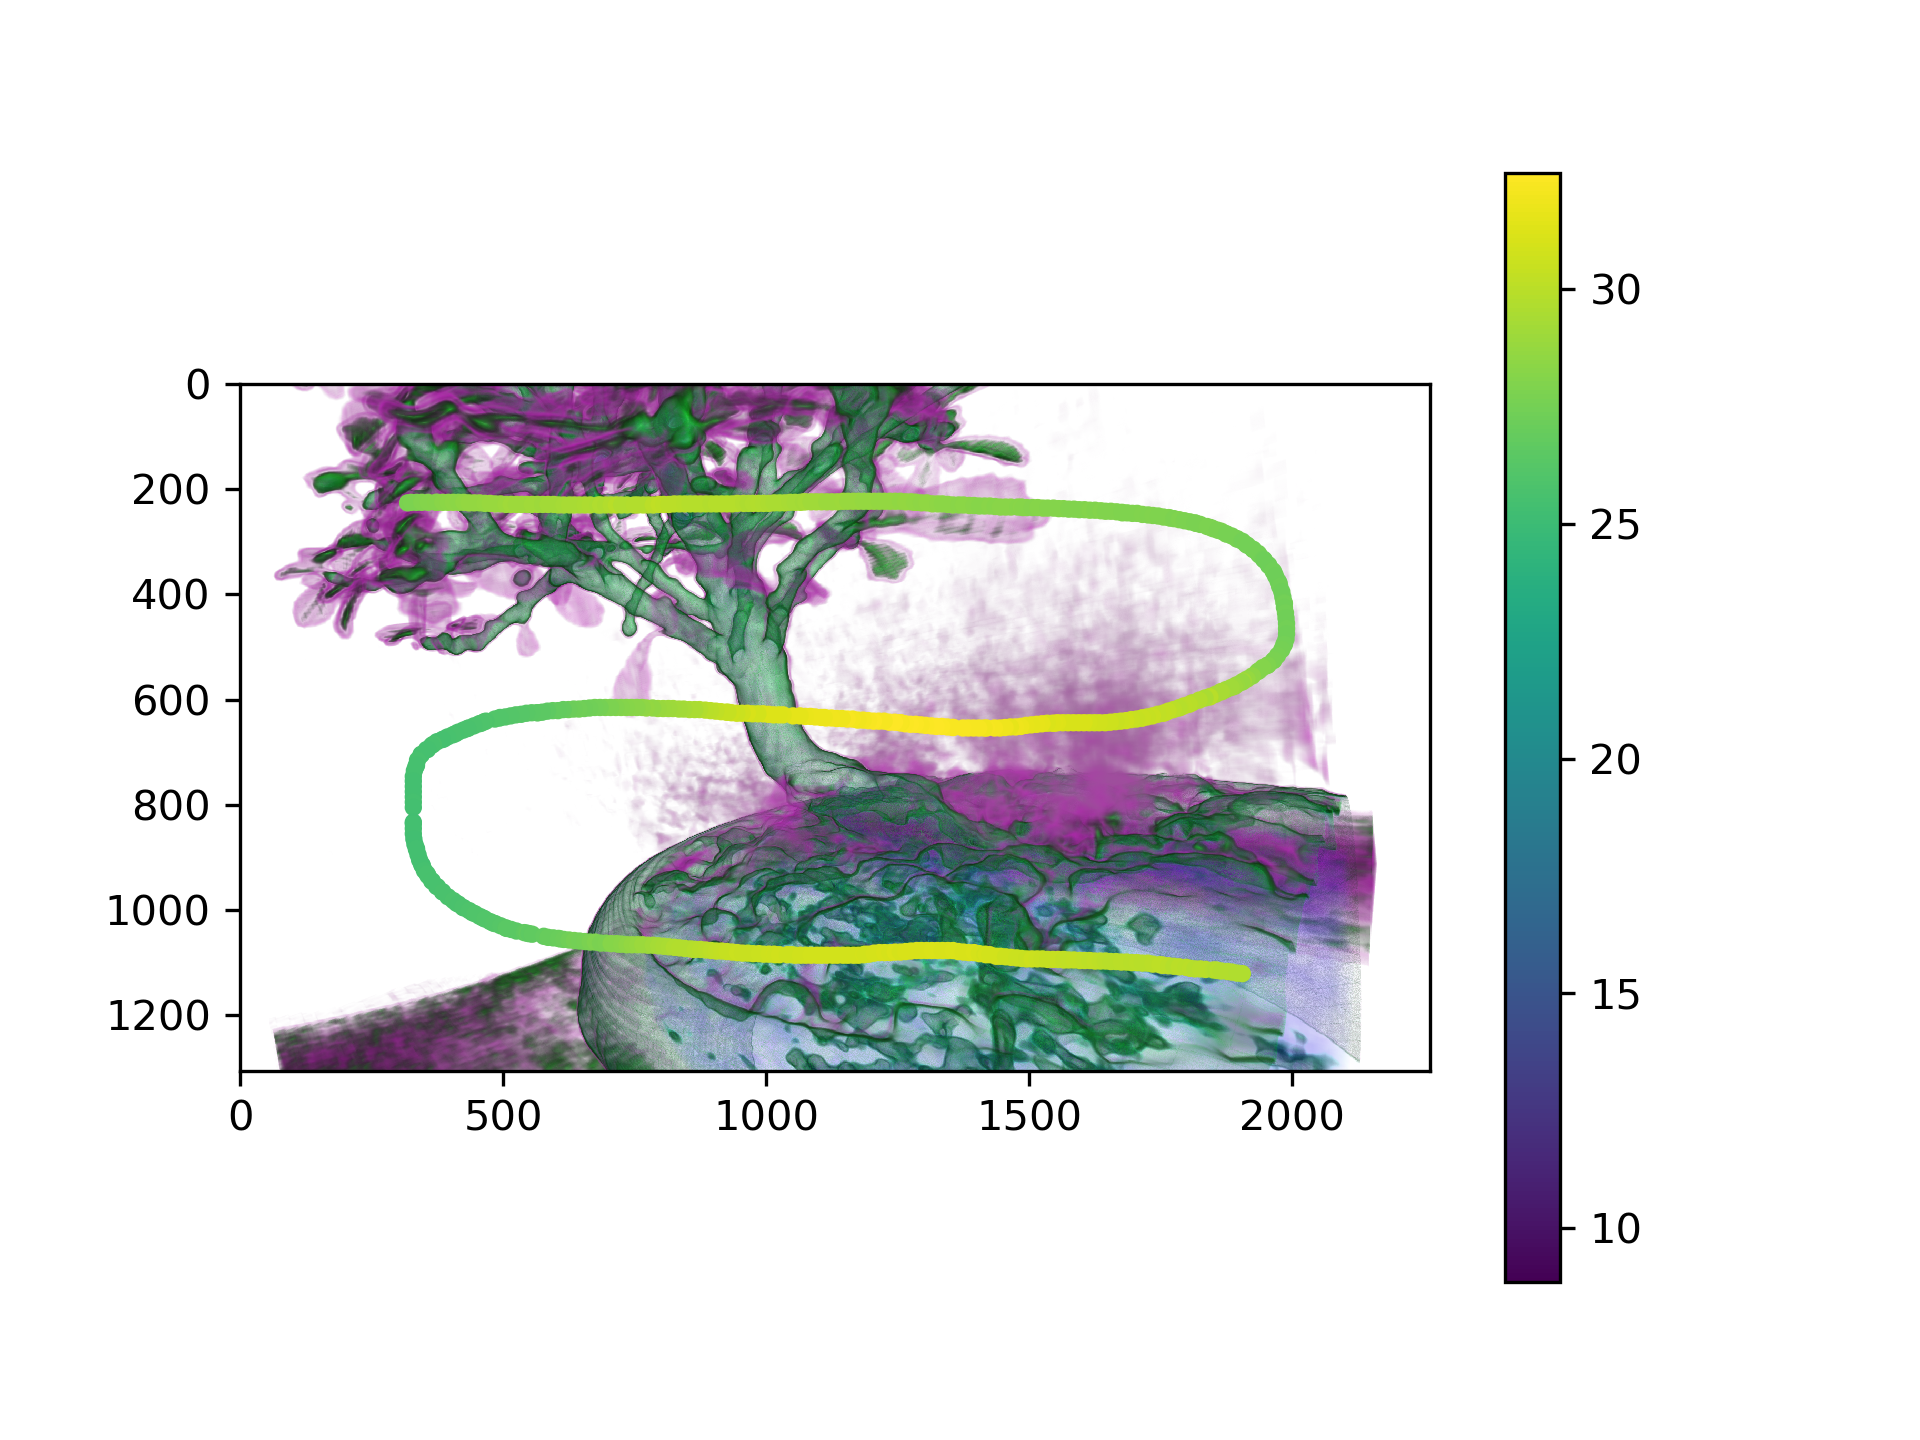
\includegraphics[width=1\textwidth]{../../Grafiken/results/performance/bonsai/ms_data_mdc_heatmap.png}
	\caption{Bonsai Heatmap \emph{MDC}.}
	\label{fig::res::pf::hm_bs_mdc}
\end{figure}
\begin{figure}
	\centering
	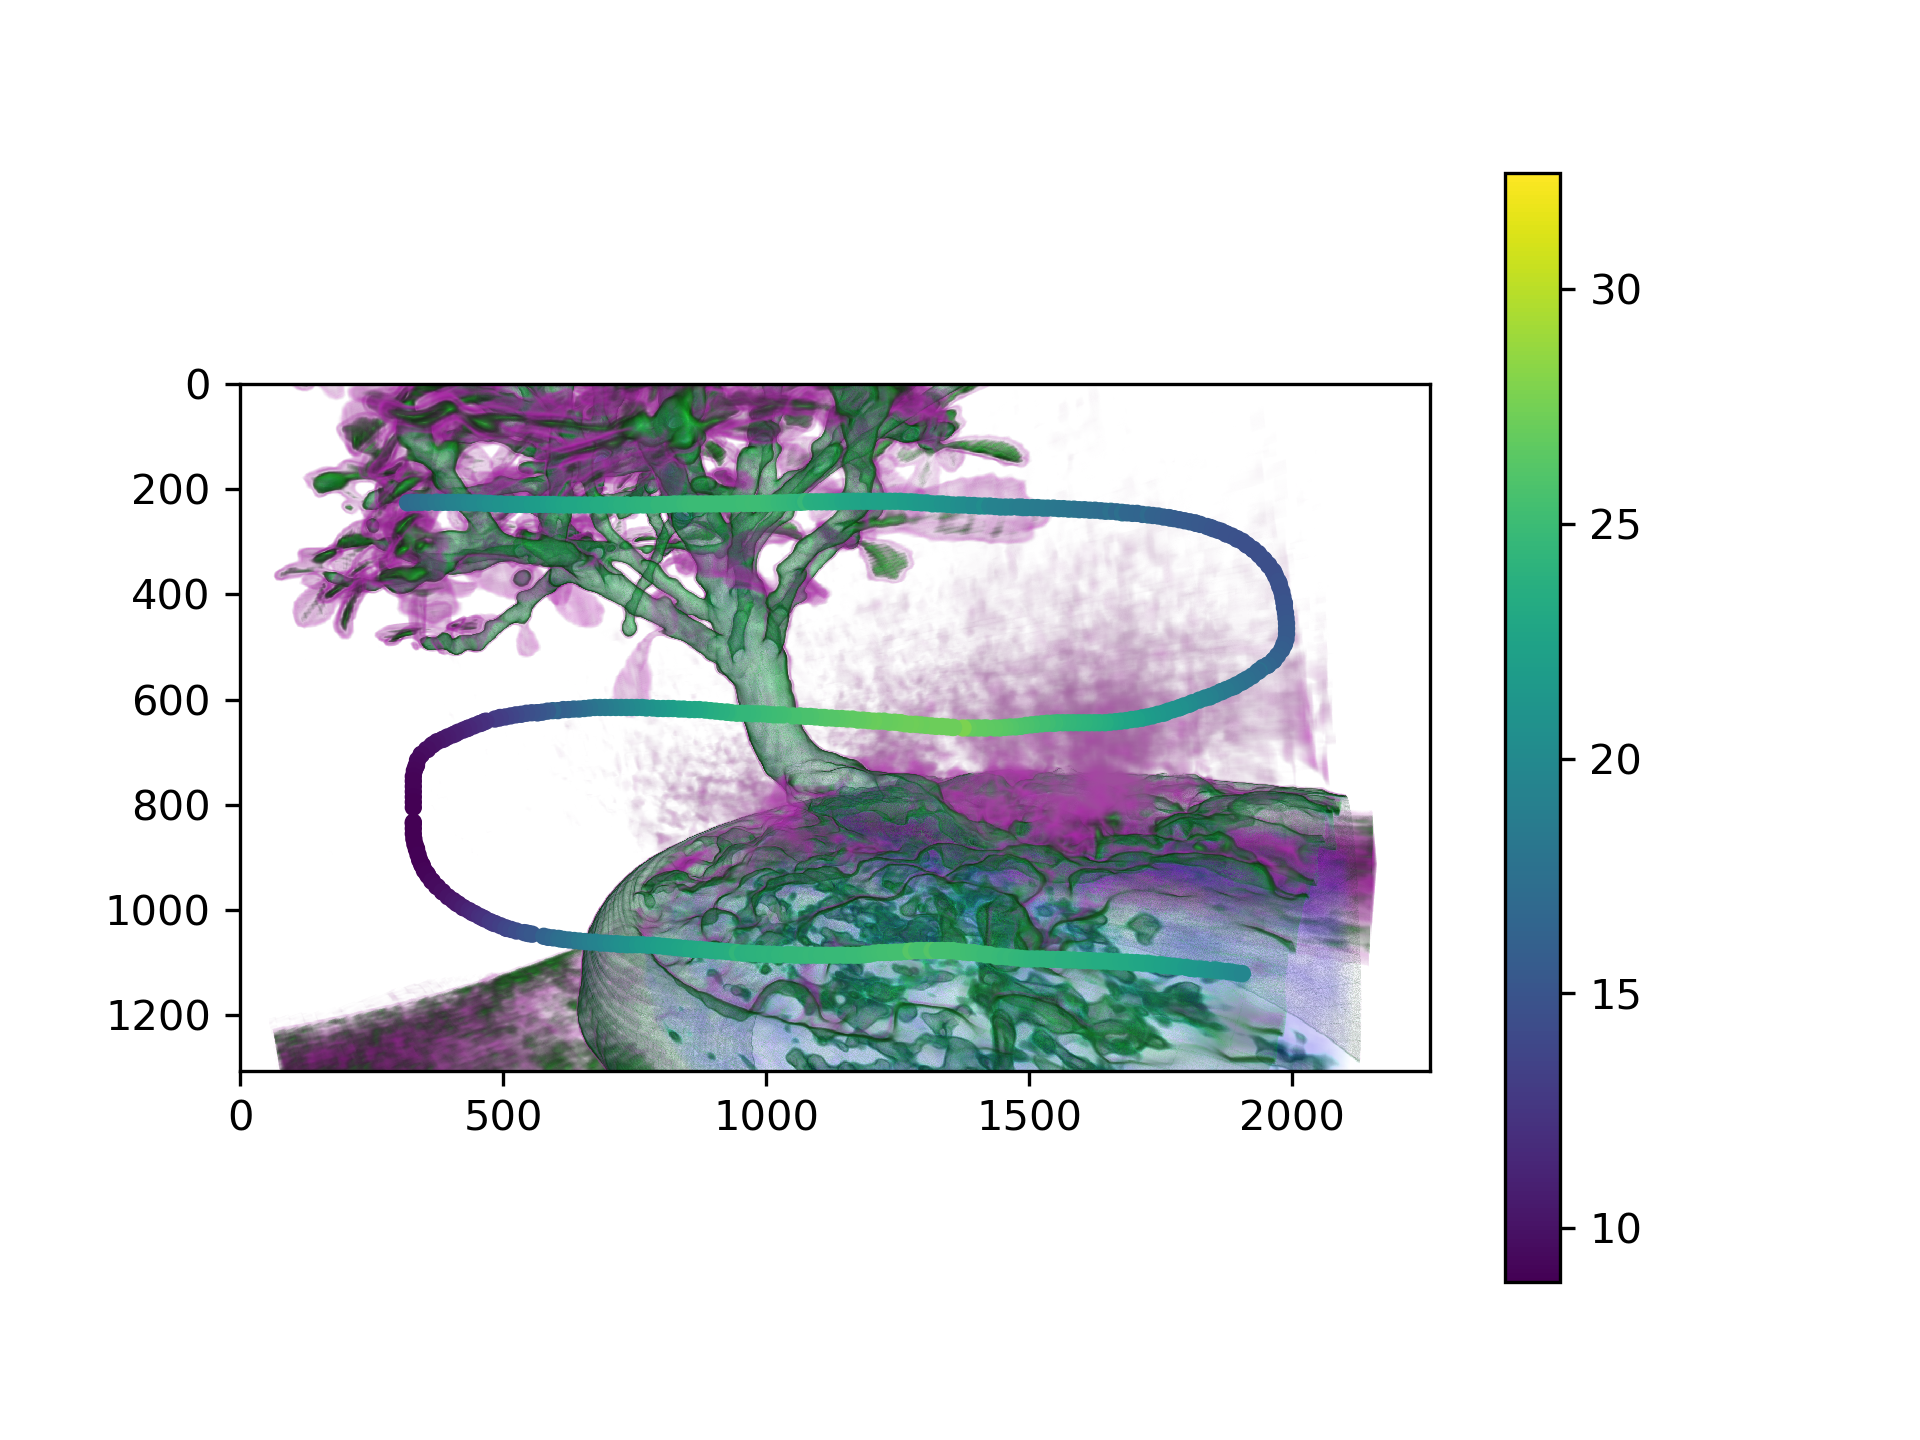
\includegraphics[width=1\textwidth]{../../Grafiken/results/performance/bonsai/ms_data_ddc_heatmap.png}
	\caption{Bonsai Heatmap \emph{DDC}.}
	\label{fig::res::pf::hm_bs_ddc}
\end{figure}
\begin{figure}
	\centering
	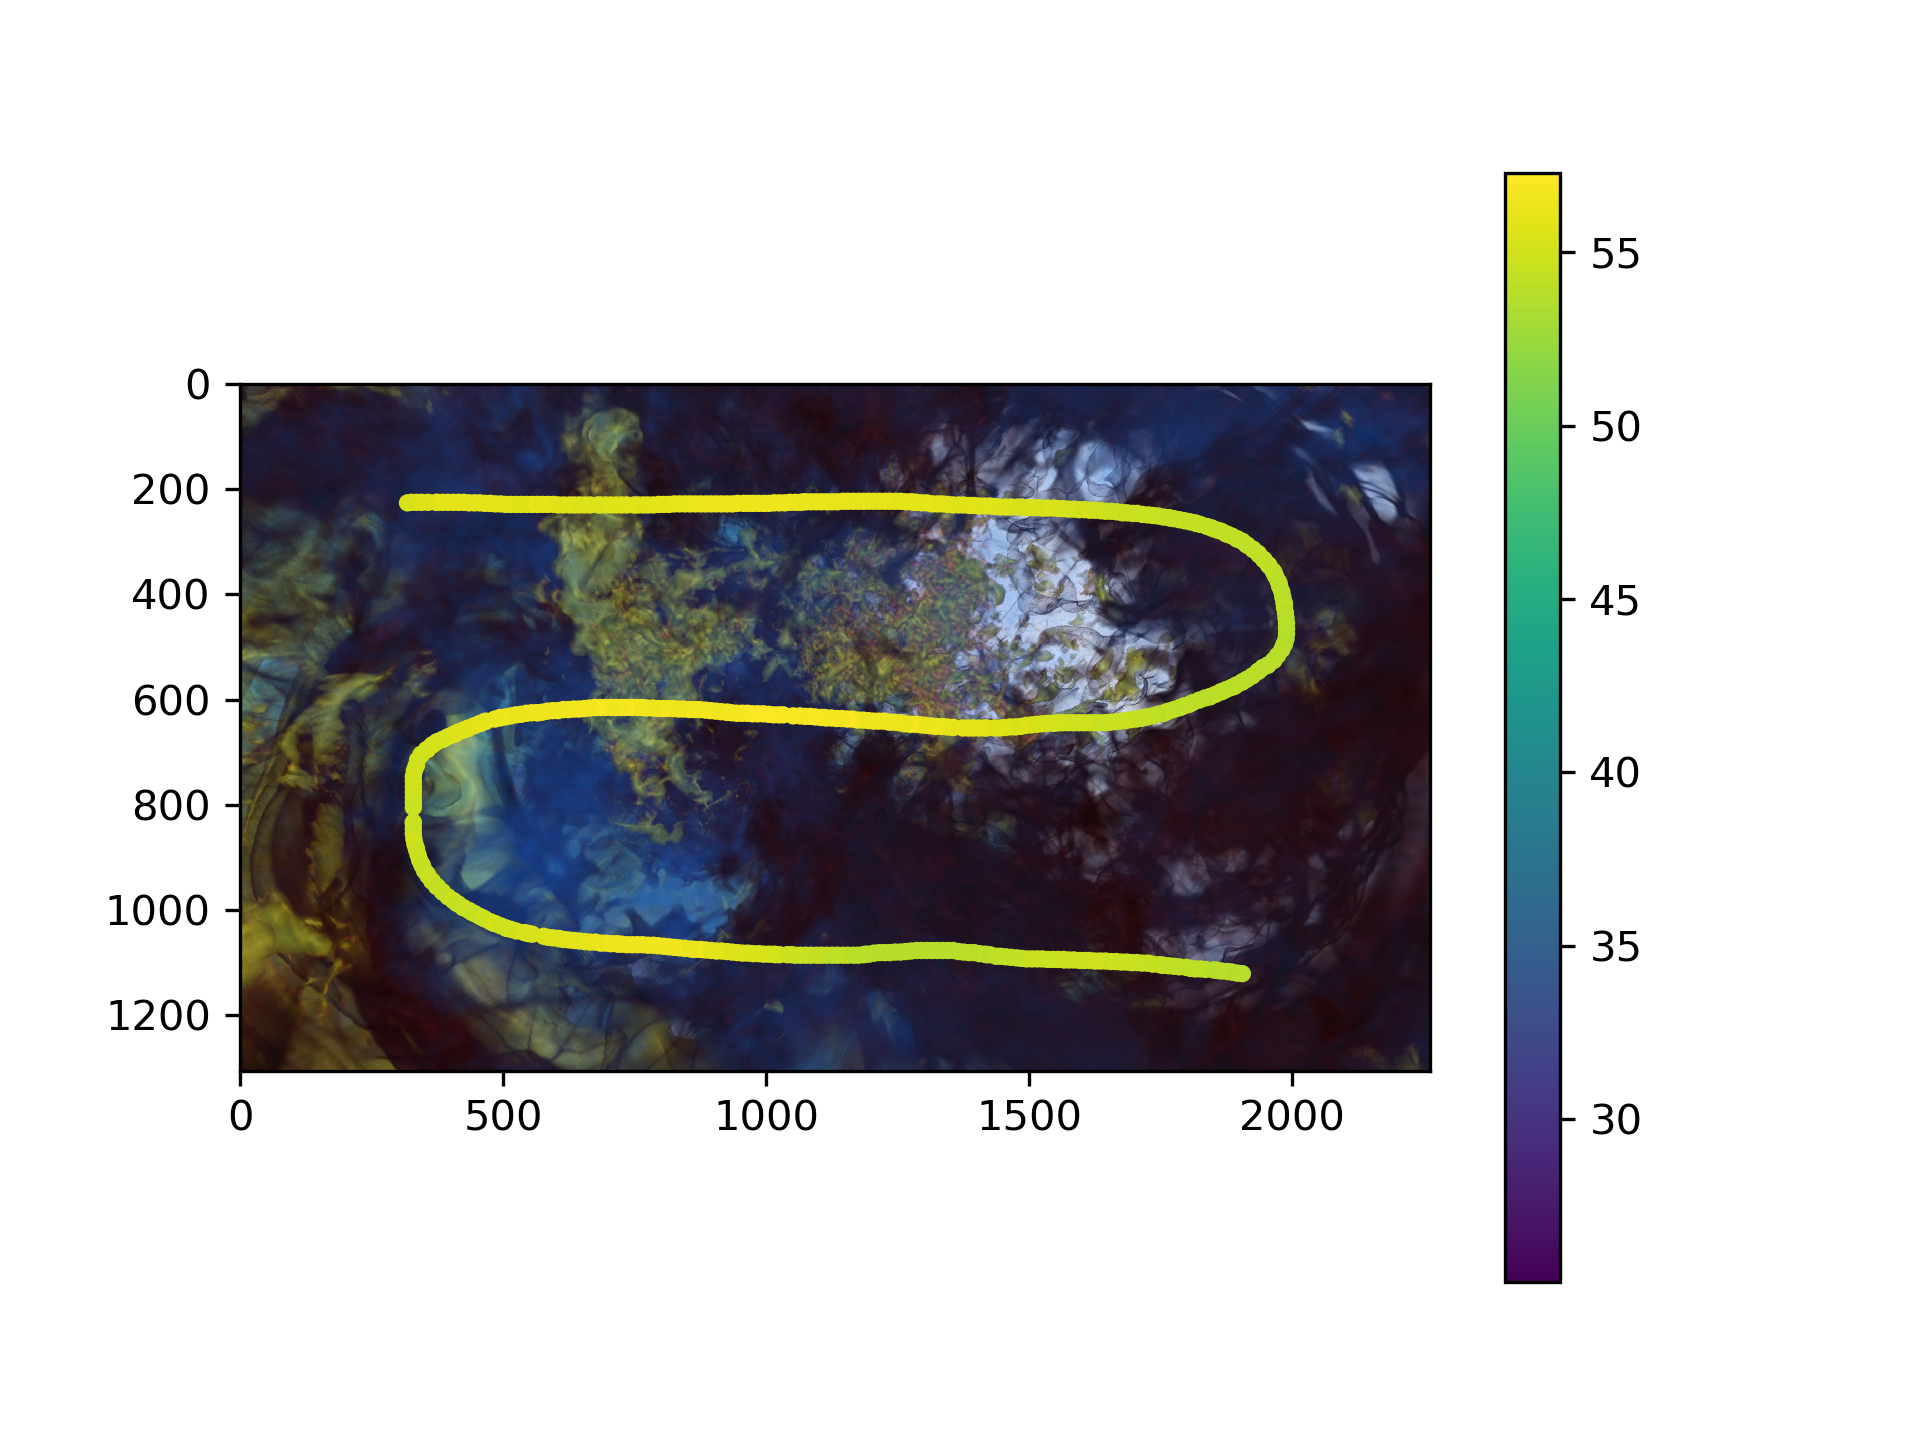
\includegraphics[width=1\textwidth]{../../Grafiken/results/performance/supernova/ms_data_mdc_heatmap.png}
	\caption{Supernova Heatmap \emph{MDC}.}
	\label{fig::res::pf::hm_sn_mdc}
\end{figure}
\begin{figure}
	\centering
	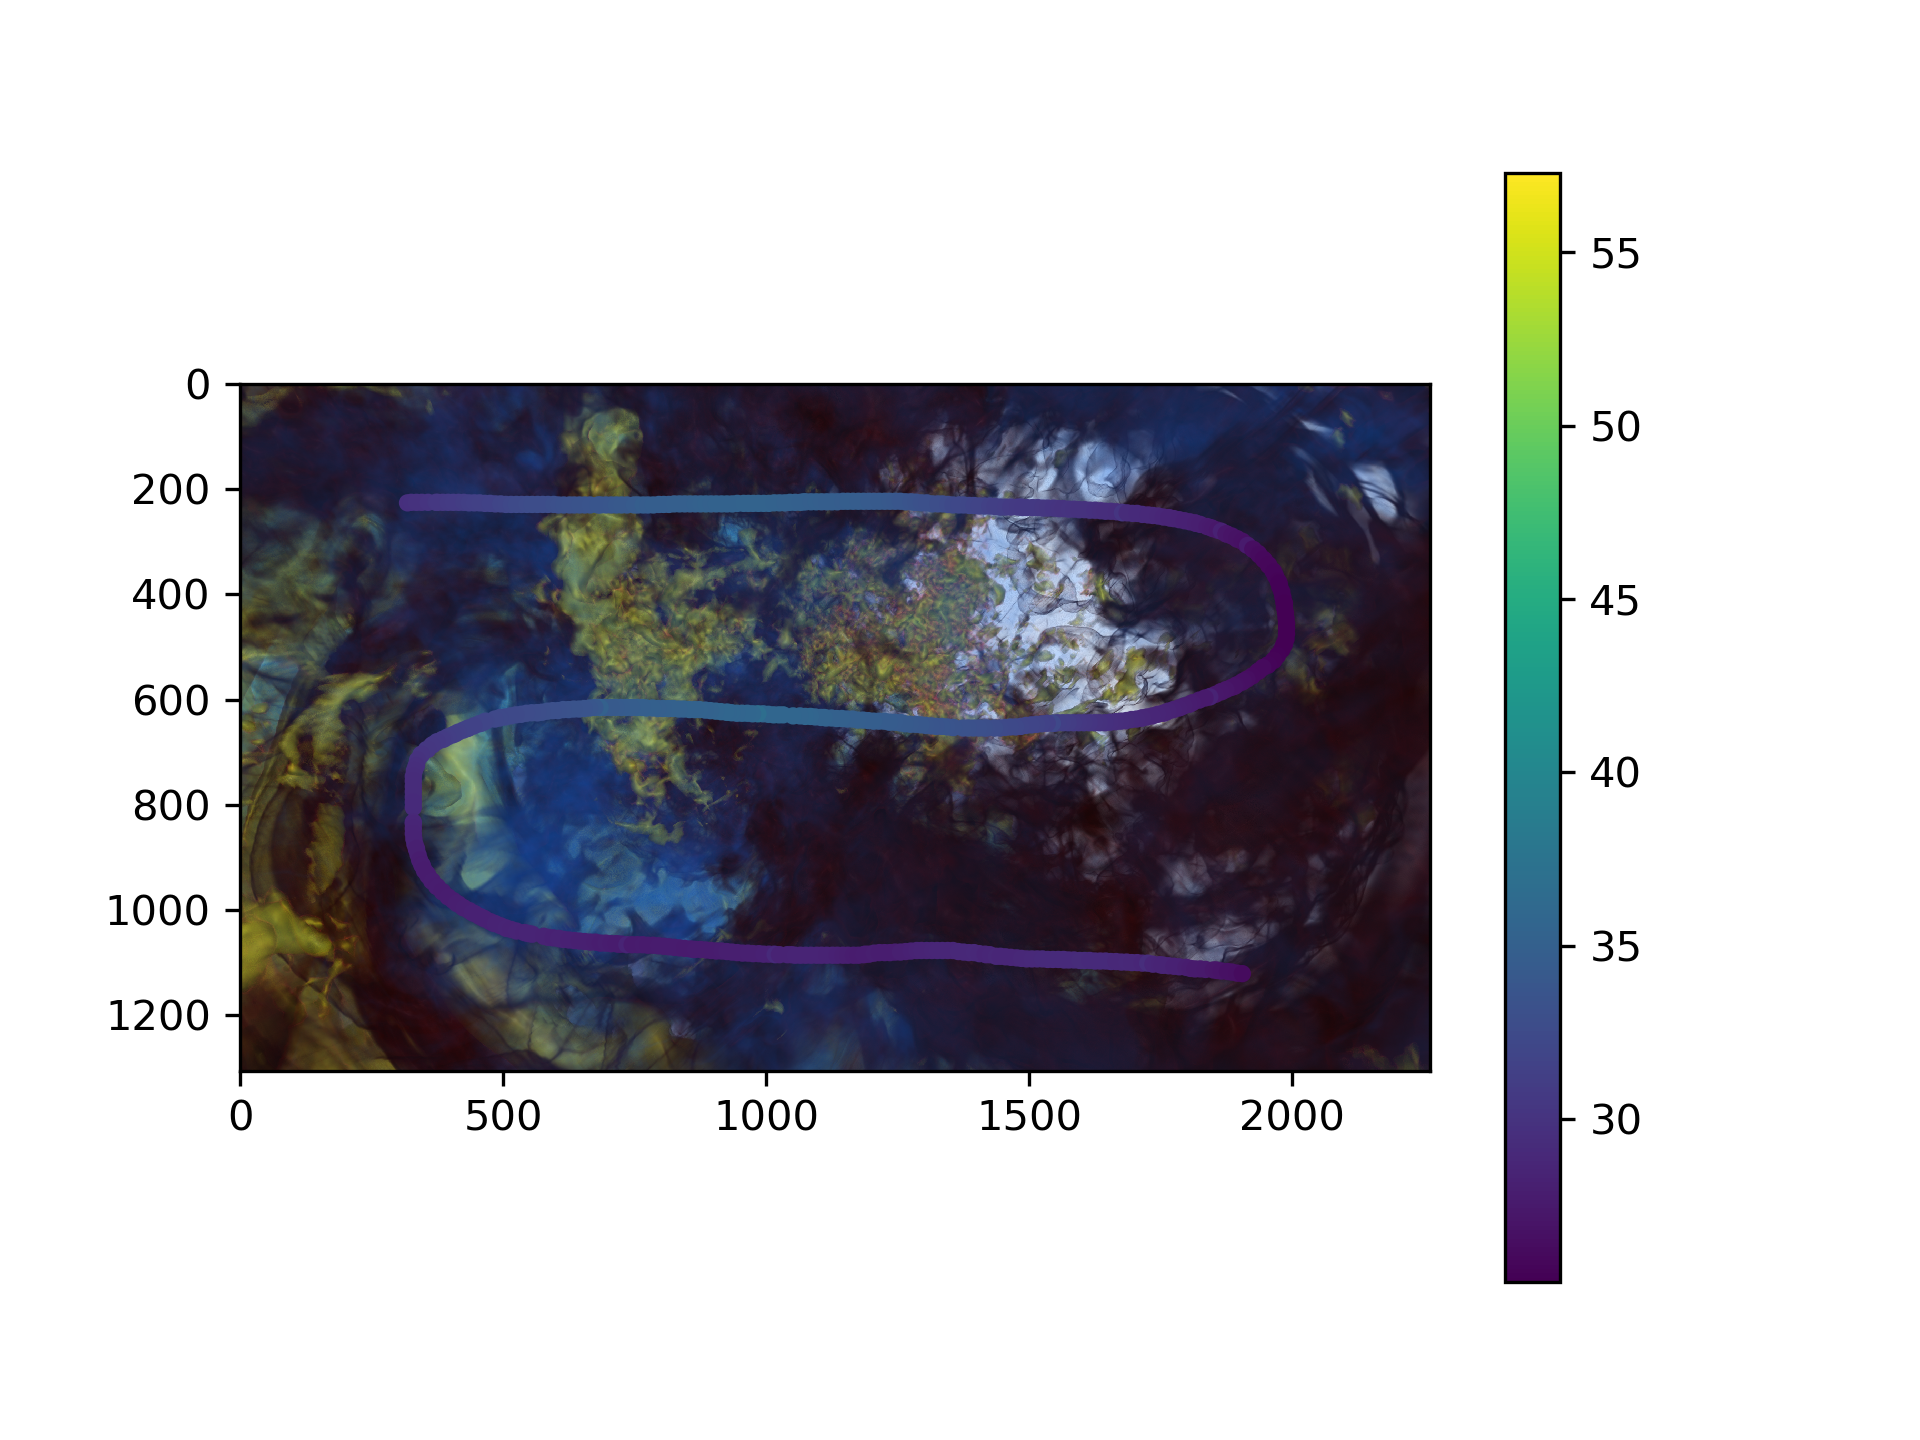
\includegraphics[width=1\textwidth]{../../Grafiken/results/performance/supernova/ms_data_ddc_heatmap.png}
	\caption{Supernova Heatmap \emph{DDC}.}
	\label{fig::res::pf::hm_sn_ddc}
\end{figure}

\cleardoublepage

\subsection{Transferfunktion und Renderoptionen}
\todo{Ergebnisse zur Nutzung der Transferfunktion, Interpolation, Ambient Occlusion und Orthografische Ansicht.}

\section*{Diskussion}\label{sec::disc}
\todo{Technische Daten des Systems, mit dem das Eyetracking gemacht wurde, angeben. Am besten die wichtigen Messungen mit dem Eye Tracker PC wiederholen.}
\todo{Diskussion und Bedeutung der Ergebnisse.}